\documentclass[12pt,twoside]{article}
%\date{}   %uncommenting this erases the date
\usepackage{graphicx}
\usepackage{amsmath}
\usepackage{amssymb}
%\usepackage{natbib}
%\usepackage{verbatim}
\usepackage{floatpag}
\usepackage{subeqnarray}
\usepackage{mathrsfs}    %for special characters
\usepackage{cancel}  % to set terms in an equation to zero
\usepackage{caption}
\usepackage{subcaption}


\setlength{\textheight}     {9.0in}
\setlength{\textwidth}      {6.5in}
\setlength{\oddsidemargin}  {0.0in}
\setlength{\evensidemargin} {0.0in}
\setlength{\topmargin}      {0.0in}
\setlength{\headheight}     {0.0in}
\setlength{\headsep}        {0.0in}
\setlength{\hoffset}        {0.0in}
\setlength{\voffset}        {0.0in}
\setlength{\parindent}      {0.0in}      %starting new line at extreme left

\graphicspath{{Figures/}}

\newcommand{\astrut}{\usebox{\astrutbox}}

\newcommand\GaPQ{\ensuremath{G_a(P,Q)}}
\newcommand\GsPQ{\ensuremath{G_s(P,Q)}}
\newcommand\p{\ensuremath{\partial}}
\newcommand\tti{\ensuremath{\rightarrow\infty}}
\newcommand\kgd{\ensuremath{k\gamma d}}
\newcommand\shalf{\ensuremath{{\scriptstyle\frac{1}{2}}}}
\newcommand\sh{\ensuremath{^{\shalf}}}
\newcommand\smh{\ensuremath{^{-\shalf}}}
\newcommand\squart{\ensuremath{{\textstyle\frac{1}{4}}}}
\newcommand\thalf{\ensuremath{{\textstyle\frac{1}{2}}}}
\newcommand\Gat{\ensuremath{\widetilde{G_a}}}
\newcommand\ttz{\ensuremath{\rightarrow 0}}
\newcommand\ndq{\ensuremath{\frac{\mbox{$\partial$}}{\mbox{$\partial$} n_q}}}
\newcommand\sumjm{\ensuremath{\sum_{j=1}^{M}}}
\newcommand\pvi{\ensuremath{\int_0^{\infty}%
  \mskip \ifCUPmtlplainloaded -30mu\else -33mu\fi -\quad}}

\newcommand\etal{\mbox{\textit{et al.}}}
\newcommand\etc{etc.\ }
\newcommand\eg{e.g.\ }



\newcommand{\bs}  [1]{\boldsymbol{#1}}
\newcommand{\del} {\nabla}
\newcommand{\bsh}  [1]{\boldsymbol{\hat{#1}}}
\newcommand{\ul}  {\underline}
\newcommand{\ol}  {\overline}
\newcommand{\pp} [2]{\frac{\p{#1}}{\p{#2}}}
\newcommand{\dd} [2]{\frac{d{#1}}{d{#2}}}
\newcommand{\lam}  [1]{{#1}^{\tiny{\lambda}}}
\newcommand{\conj} [1]{{#1}^*}
\newcommand{\mods} [1]{ \vert {#1} \vert ^2}



\title{Computation of vortex sheet roll-up}

\author{Raghav Singhal}

\begin{document}

\maketitle
\section{Birkhoff-Rott Equation}
Given vorticity, $\omega(\bs x)$, one can calculate the stream function, $\psi(\bs x)$ as follows:

\begin{equation}
\Delta \psi(\bs x) = \omega(\bs x)
\end{equation}
Now this can be solved to get
\begin{subequations}
\begin{align}
\psi(\bs x)&=\frac{1}{2\pi}\int\limits_D{\omega(\bs x)\ln|\bs x - \bs x'|}\\
\bs v(\bs x)&=\frac{1}{2\pi}\int\limits_D{\frac{\bs {\hat z}\times(\bs x - \bs x')}{|\bs x - \bs x'|^2}\omega(\bs x')d\bs x'}
\end{align}
Using $\omega(\bs x)d\bs x=d\Gamma(\bs x)$ and restricting the domain to be a curve $C$ we obtain   %=\Gamma'(\alpha)d\bs \alpha'$
\begin{align}
\frac{\partial x(\alpha,t)}{\partial t}& = \frac{-1}{2\pi} \int\limits_C{\frac{(y(\alpha,t)-y(\alpha',t))}{((x(t)-x(\alpha',t))^2 + (y(\alpha,t)-y(\alpha',t))^2 }}\Gamma(\alpha')d\alpha'\\
\frac{\partial y(\alpha,t)}{\partial t} &= \frac{1}{2\pi}\int\limits_C{\frac{(x(t)-x(\alpha',t))}{((x(\alpha,t)-x(\alpha',t))^2 + (y(\alpha,t)-y(\alpha',t))^2 }}\Gamma(\alpha')d\alpha'
\end{align}
\end{subequations}

\section{Desingularization of the Birkhoff-Rott equation}
Given $\delta>0$, called a smoothing parameter, we consider the equations:
\begin{subequations}
\label{mom}
\begin{align}
\frac{\partial x(\alpha,t)}{\partial t}& = \frac{-1}{2\pi} \int\limits_C{\frac{(y(\alpha,t)-y(\alpha',t))}{((x(t)-x(\alpha',t))^2 + (y(\alpha,t)-y(\alpha',t))^2 + \delta^2 }}\Gamma'(\alpha')d\alpha'\\
\frac{\partial y(\alpha,t)}{\partial t} &= \frac{1}{2\pi}\int\limits_C{\frac{(x(\alpha,t)-x(\alpha',t))}{((x(\alpha,t)-x(\alpha',t))^2 + (y(\alpha,t)-y(\alpha',t))^2 + \delta^2 }}\Gamma'(\alpha')d\alpha'\end{align}
\end{subequations}
These are called the $\delta$-equations, which is an approximation to the Birkhoff-Rott equation. Our goal here is to solve the $\delta$-equations numerically and observe its behaviour as $\delta$ approaches 0. 

\section{Discretization}

We apply standard discretization techniques to solve the $\delta$-equations.Let $z_j$(t)=$x_j$(t)+$iy_j$(t) be an approximation to the vortex sheet's position $z(\Gamma(\alpha_j),t)$ at equidistant parameter values $\alpha_j$=$\pi(j-1)/2N$ , $j=1,2.....2N+1$. The integral is evaluated by the trapezoidal rule, yielding a system of coupled ordinary differential equations for the blob's motions:

\begin{subequations}
\begin{align}
\frac{d x_j}{d t} = \sum_{k=1}^{2N+1}{\frac{-(y_j(t)-y_k(t))}{((x_j(t)-x_k(t))^2 + (y_j(t)-y_k(t))^2 + \delta^2)}}w_k\\
\frac{d y_j}{d t} = \sum_{k=1}^{2N+1}{\frac{(x_j(t)-x_k(t))}{((x_j(t)-x_k(t))^2 + (y_j(t)-y_k(t))^2 + \delta^2)}}w_k
\end{align}
\end{subequations}
where $w_k=\Gamma'(\alpha_k)\frac{1}{2\pi N},k=1,2.....2N+1$ refer to the quadrature weights. We use the fourth-order Runge Kutta scheme to integrate the above system of equations.
\section{Periodic Vortex Sheet}
The $\delta$-equations for a periodic vortex-sheet are given by:
\begin{subequations}
\begin{align}
\frac{d x_j}{d t}  =\frac{-1}{2N} \sum_{{\substack{k=1 \\ k\neq j}}}^{N}{\frac{\sinh2\pi(y_j(t)-y_k(t))}{(\cosh2\pi(x_j(t)-x_k(t)) - \cos2\pi(y_j(t)-y_k(t)) + \delta^2)}}w_k\\
\frac{d y_j}{d t}=\frac{1}{2N} \sum_{{\substack{k=1 \\ k\neq j}}}^{N}{\frac{\sin2\pi(x_j(t)-x_k(t))}{(\cosh2\pi(x_j(t)-x_k(t)) - \cos2\pi(y_j(t)-y_k(t)) + \delta^2)}}w_k
\end{align}
\end{subequations}
The initial conditions are given by
$x_j(0)=\Gamma_j+0.01\sin2\pi\Gamma_j$and $y_j(0)=-0.01\sin2\pi\Gamma_j$ . 

The figures below show a trignometric interpolating polynomial, in the variable $\Gamma$. It interpolates the perturbation quantities $p_j(t)=x_j(t)-\Gamma_j + iy_j(t)$, the coefficients of the polynomial are the fourier coefficients of $p_j$ and are calculated using the Fast Fourier Transform. The plotted image is $\Gamma + P(\Gamma,t)$, where P is the polynomial described above.

\begin{figure}
\begin{center}
	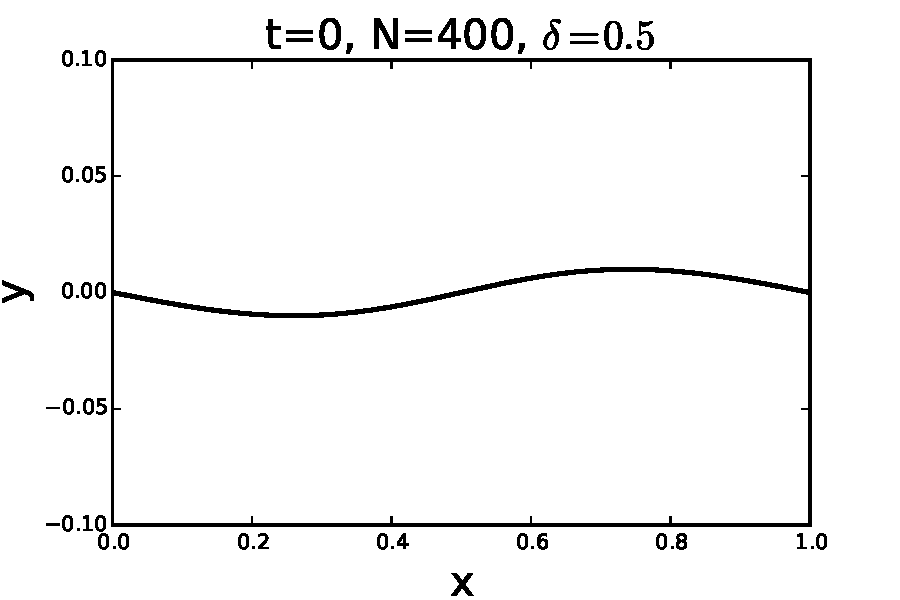
\includegraphics[width=2in,height=1.33in]{K1.pdf}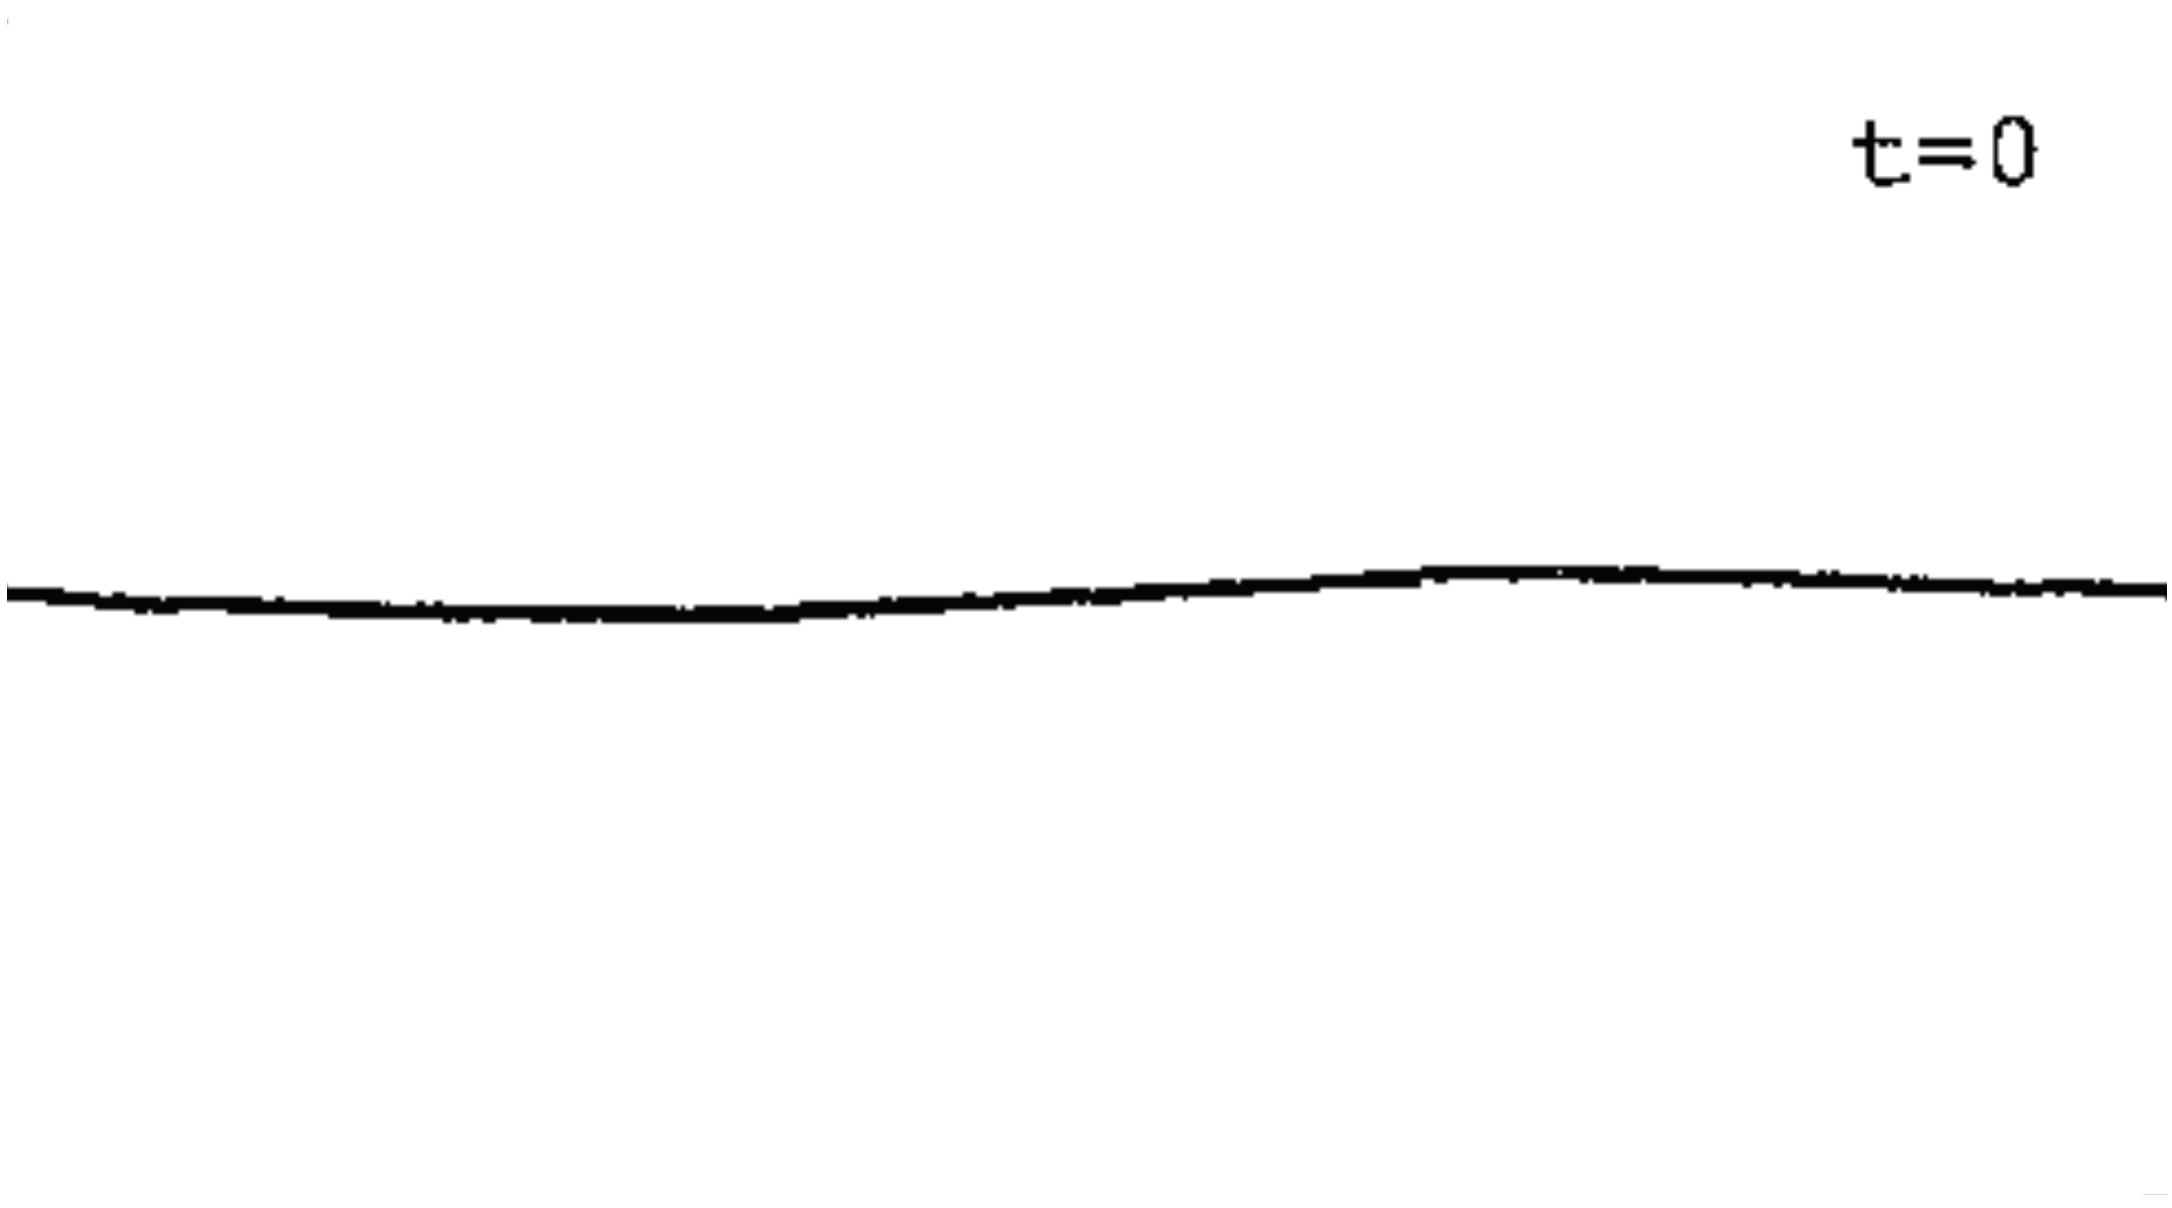
\includegraphics[width=1.5in,height=1.2in]{periodic1.png}\\
	
	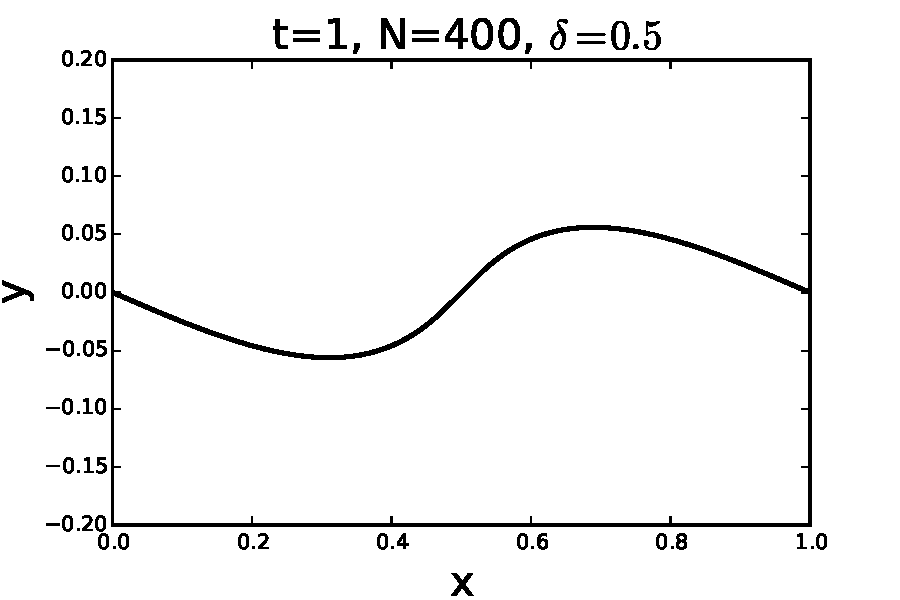
\includegraphics[width=2in,height=1.33in]{K2.pdf}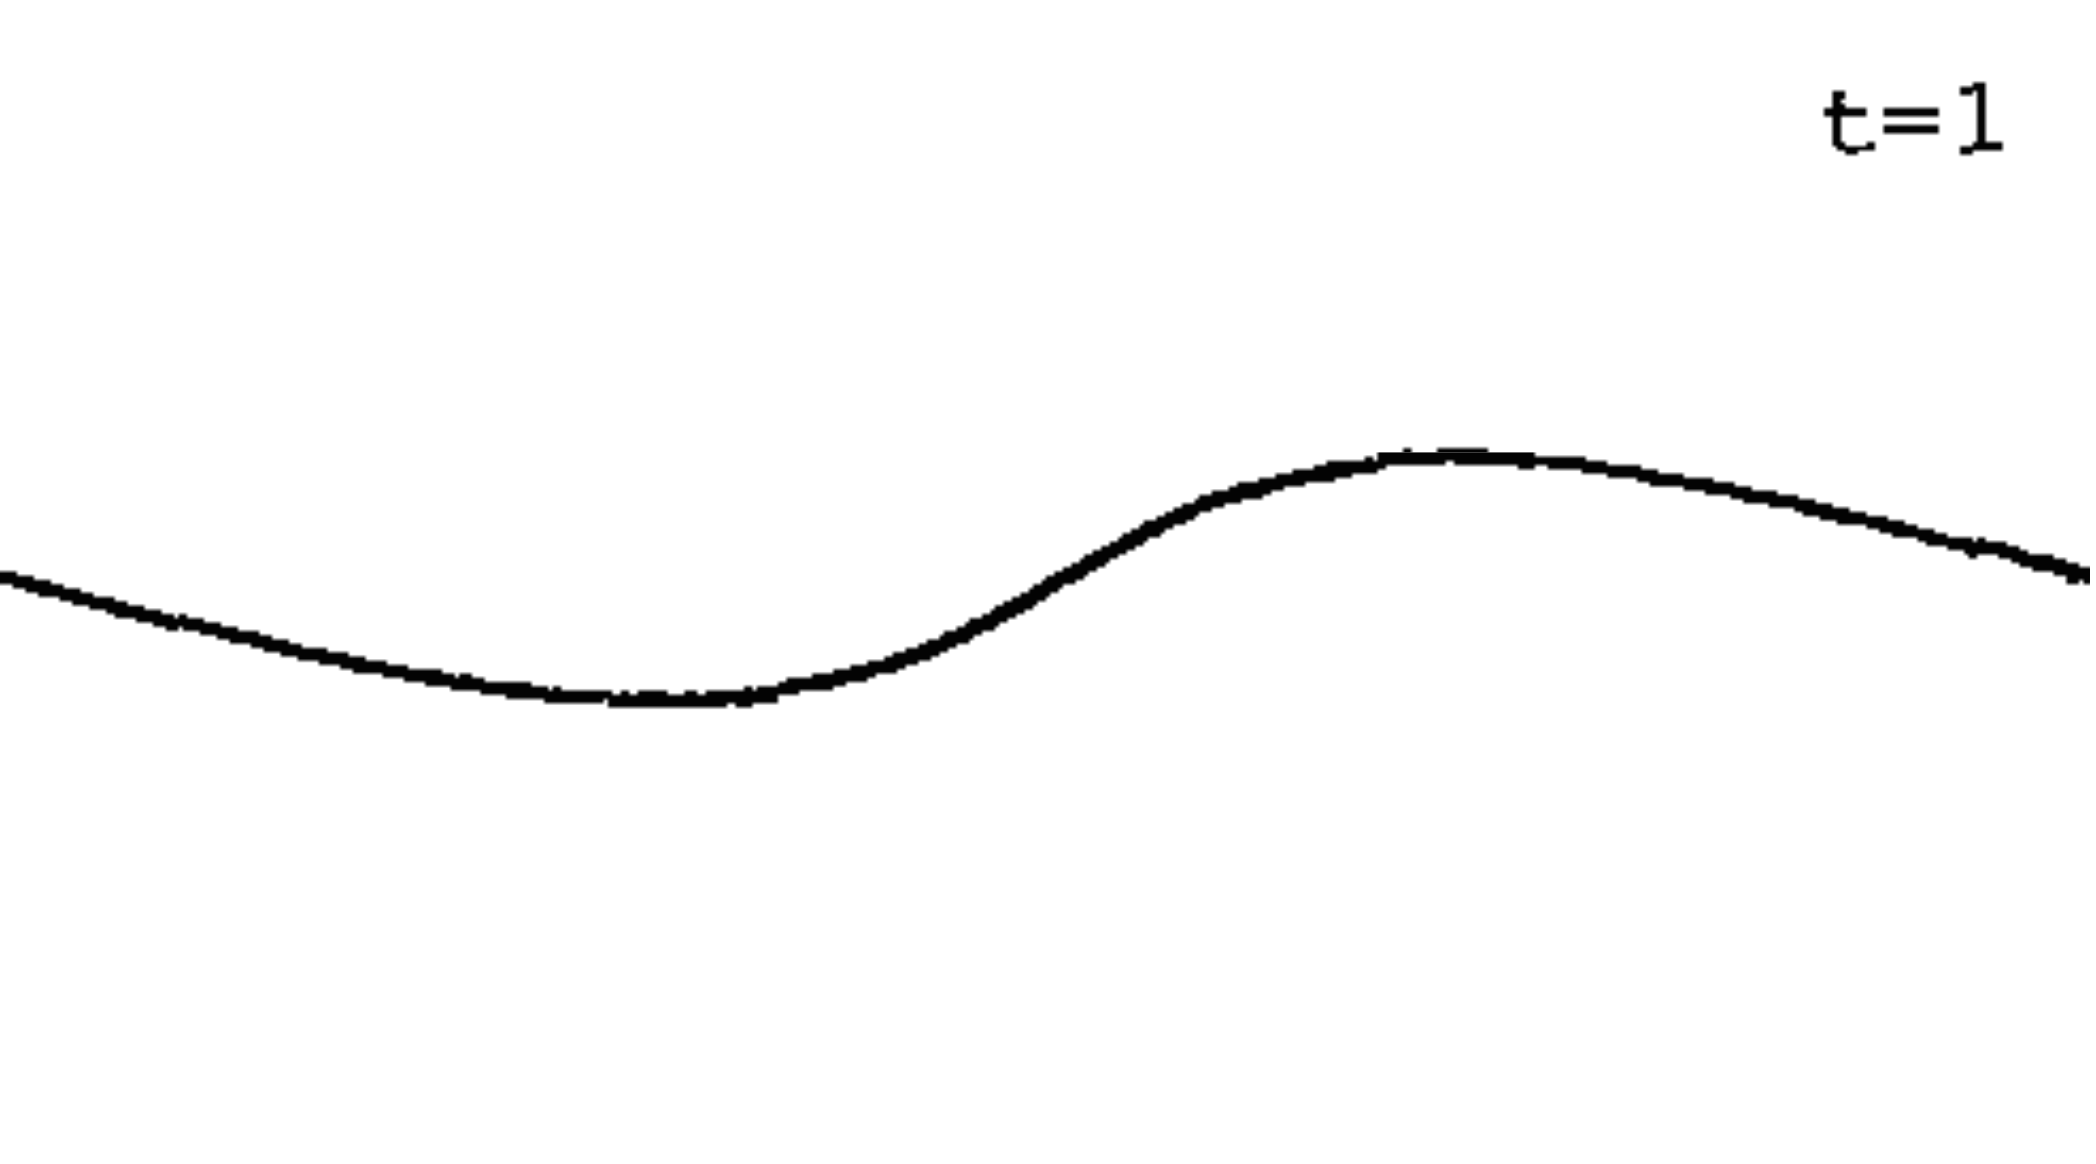
\includegraphics[width=1.5in,height=1.1in]{periodic2.png}\\
	
	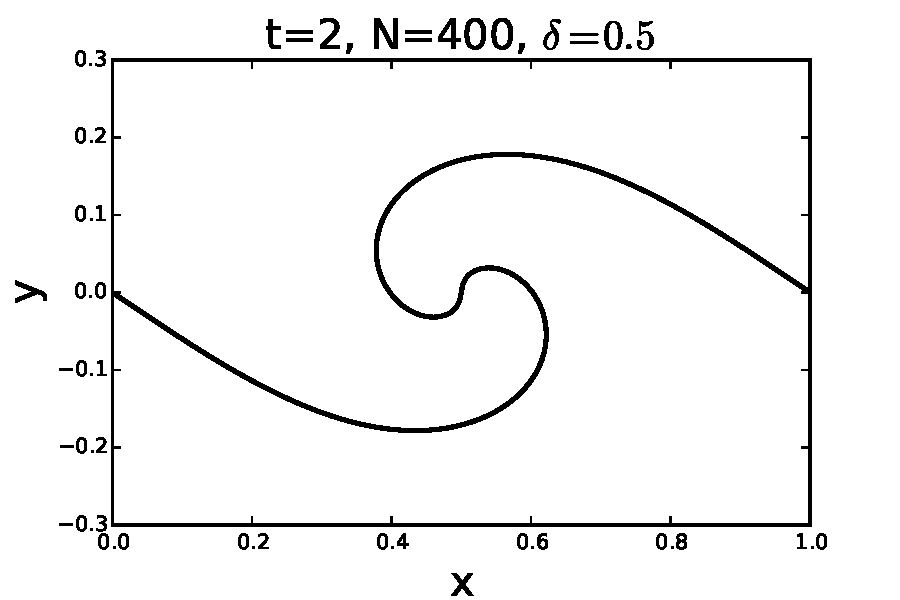
\includegraphics[width=2in,height=1.33in]{K3.pdf}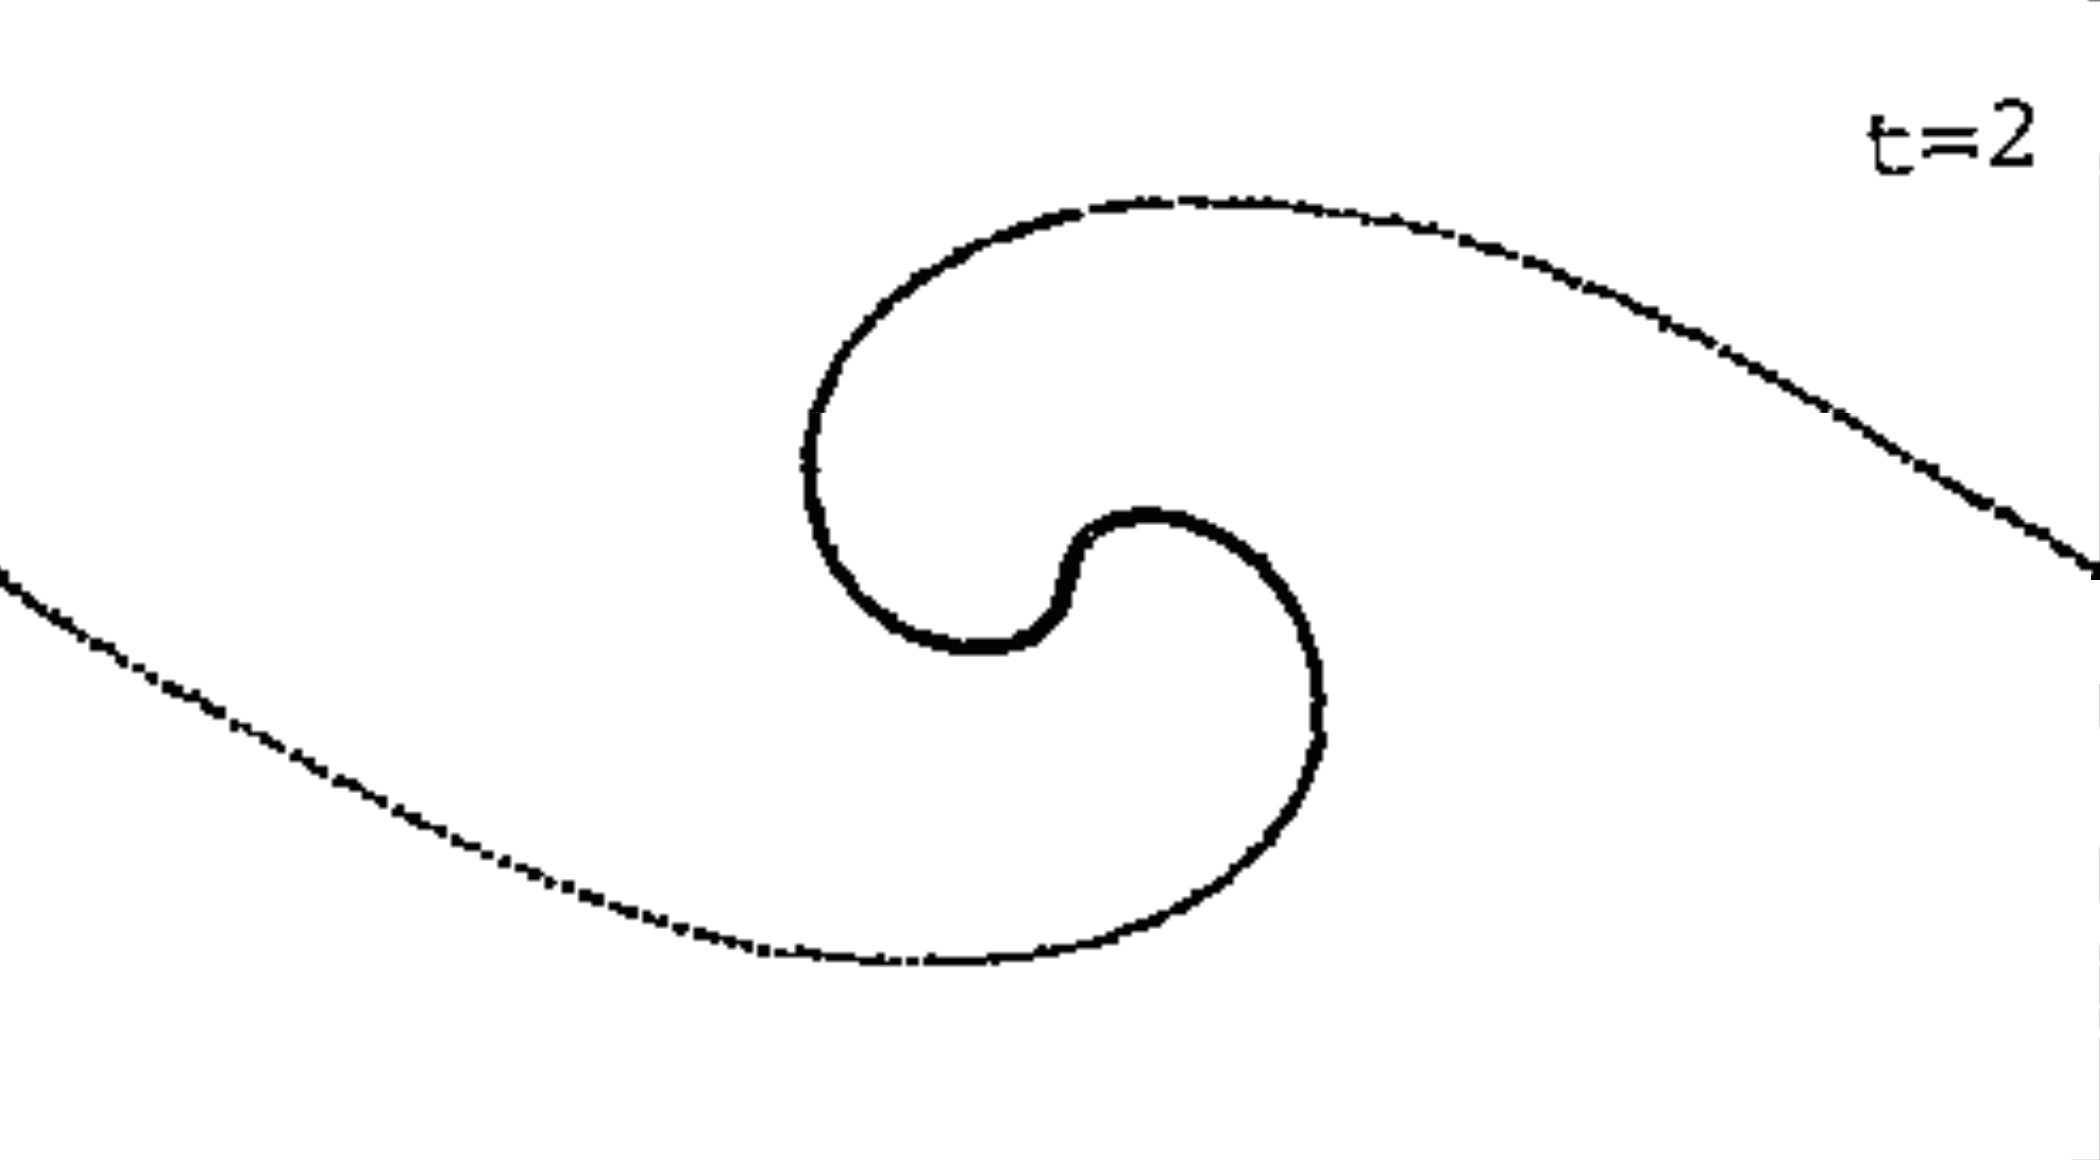
\includegraphics[width=1.5in,height=1.2in]{periodic3.png}
	
	\includegraphics[width=2in,height=1.33in]{K4.pdf}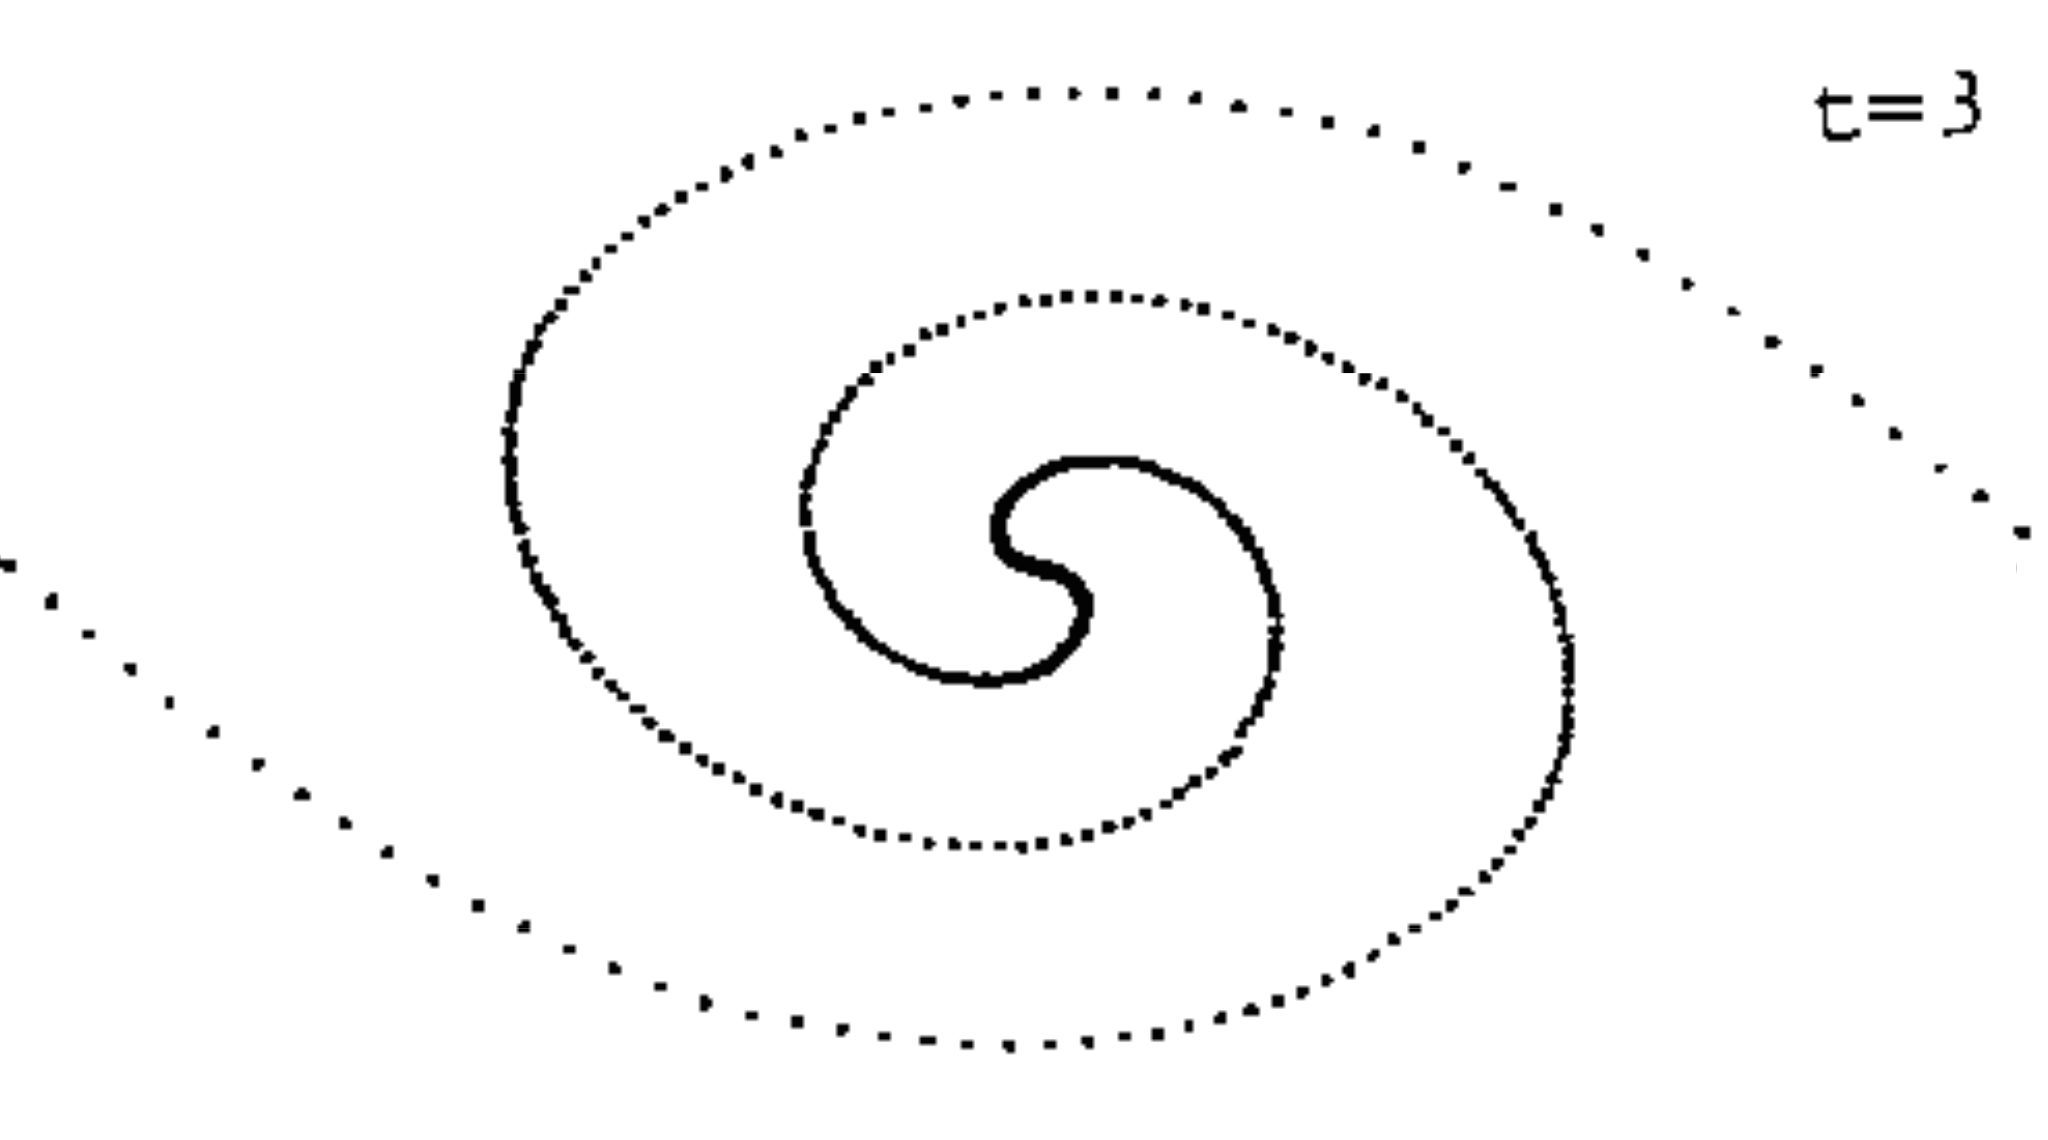
\includegraphics[width=1.5in,height=1.2in]{periodic4.png}
	
	\includegraphics[width=2in,height=1.33in]{K5.pdf}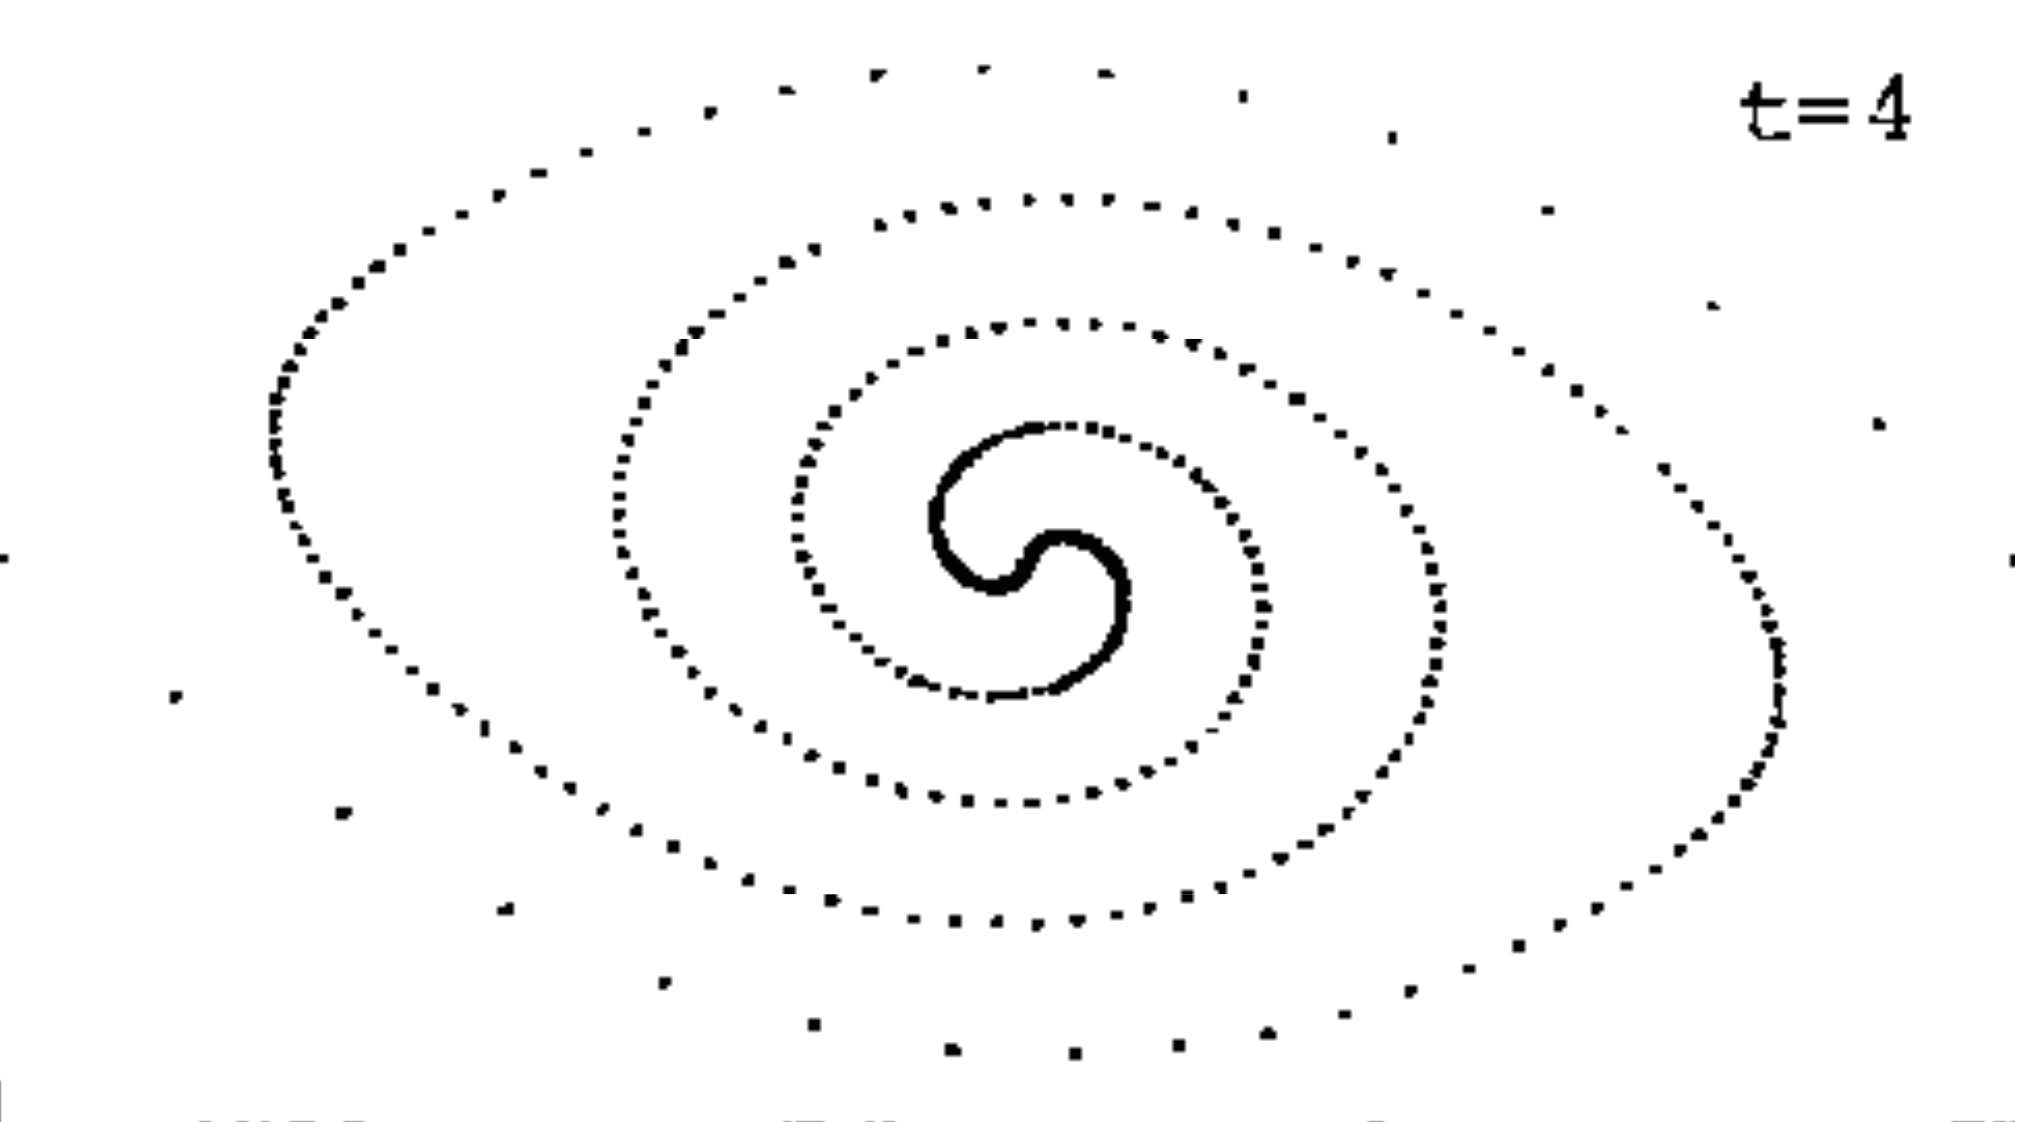
\includegraphics[width=1.5in,height=1.2in]{periodic5.png}
\end{center}
\caption{Periodic Vortex-Sheet Roll-up, with $N=400$, $\delta=0.5$ and $\Delta t=0.1$}
\label{sw2}
\end{figure}
\begin{figure}
\begin{center}
	\includegraphics[width=2in,height=1.33in]{K6.pdf}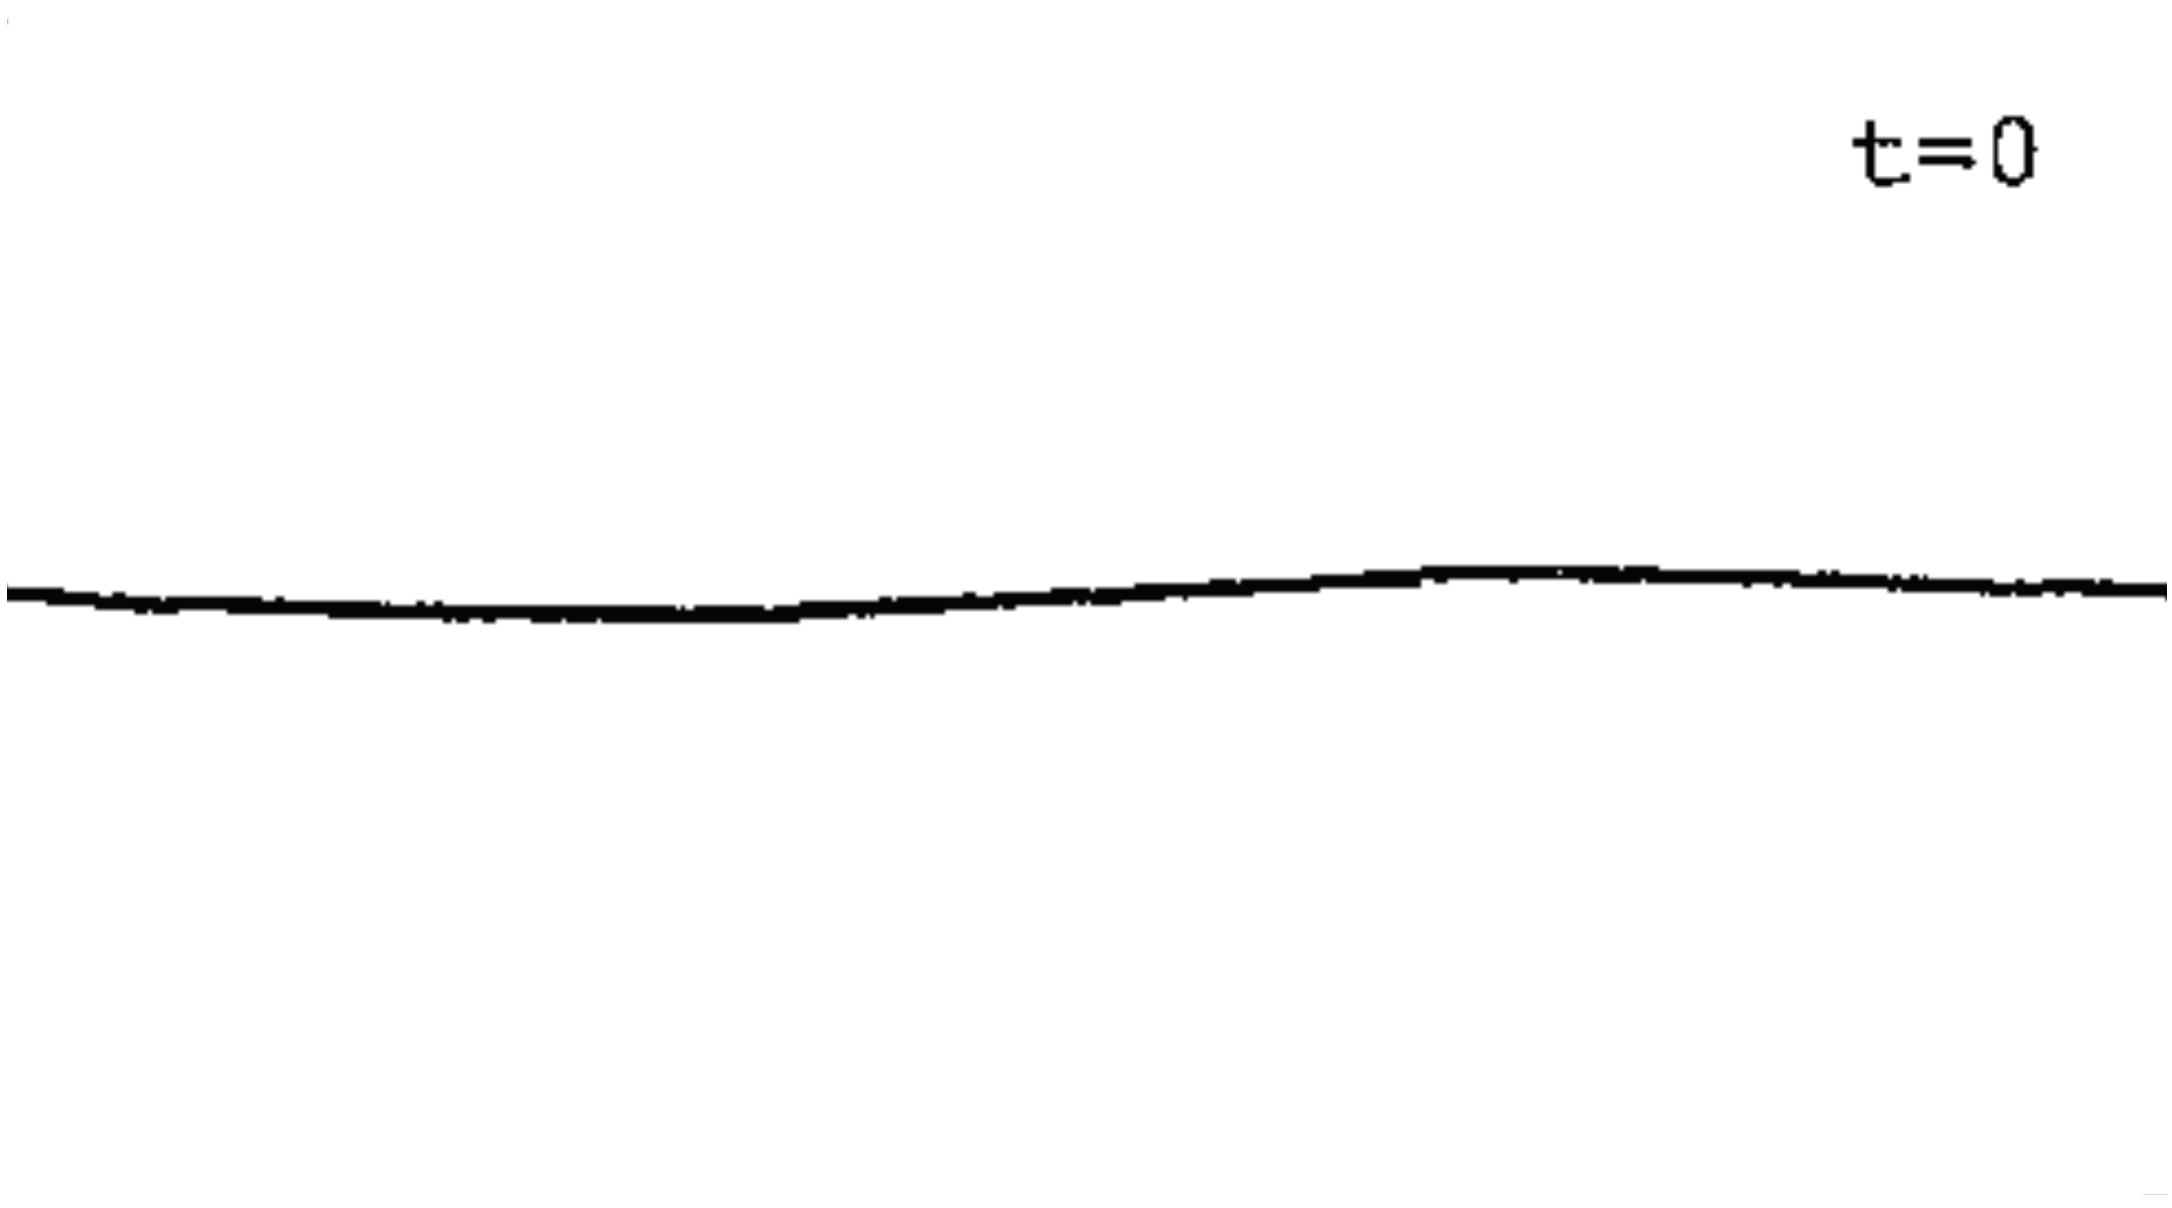
\includegraphics[width=1.5in,height=1.2in]{periodic1.png}

	\includegraphics[width=2in,height=1.33in]{K7.pdf}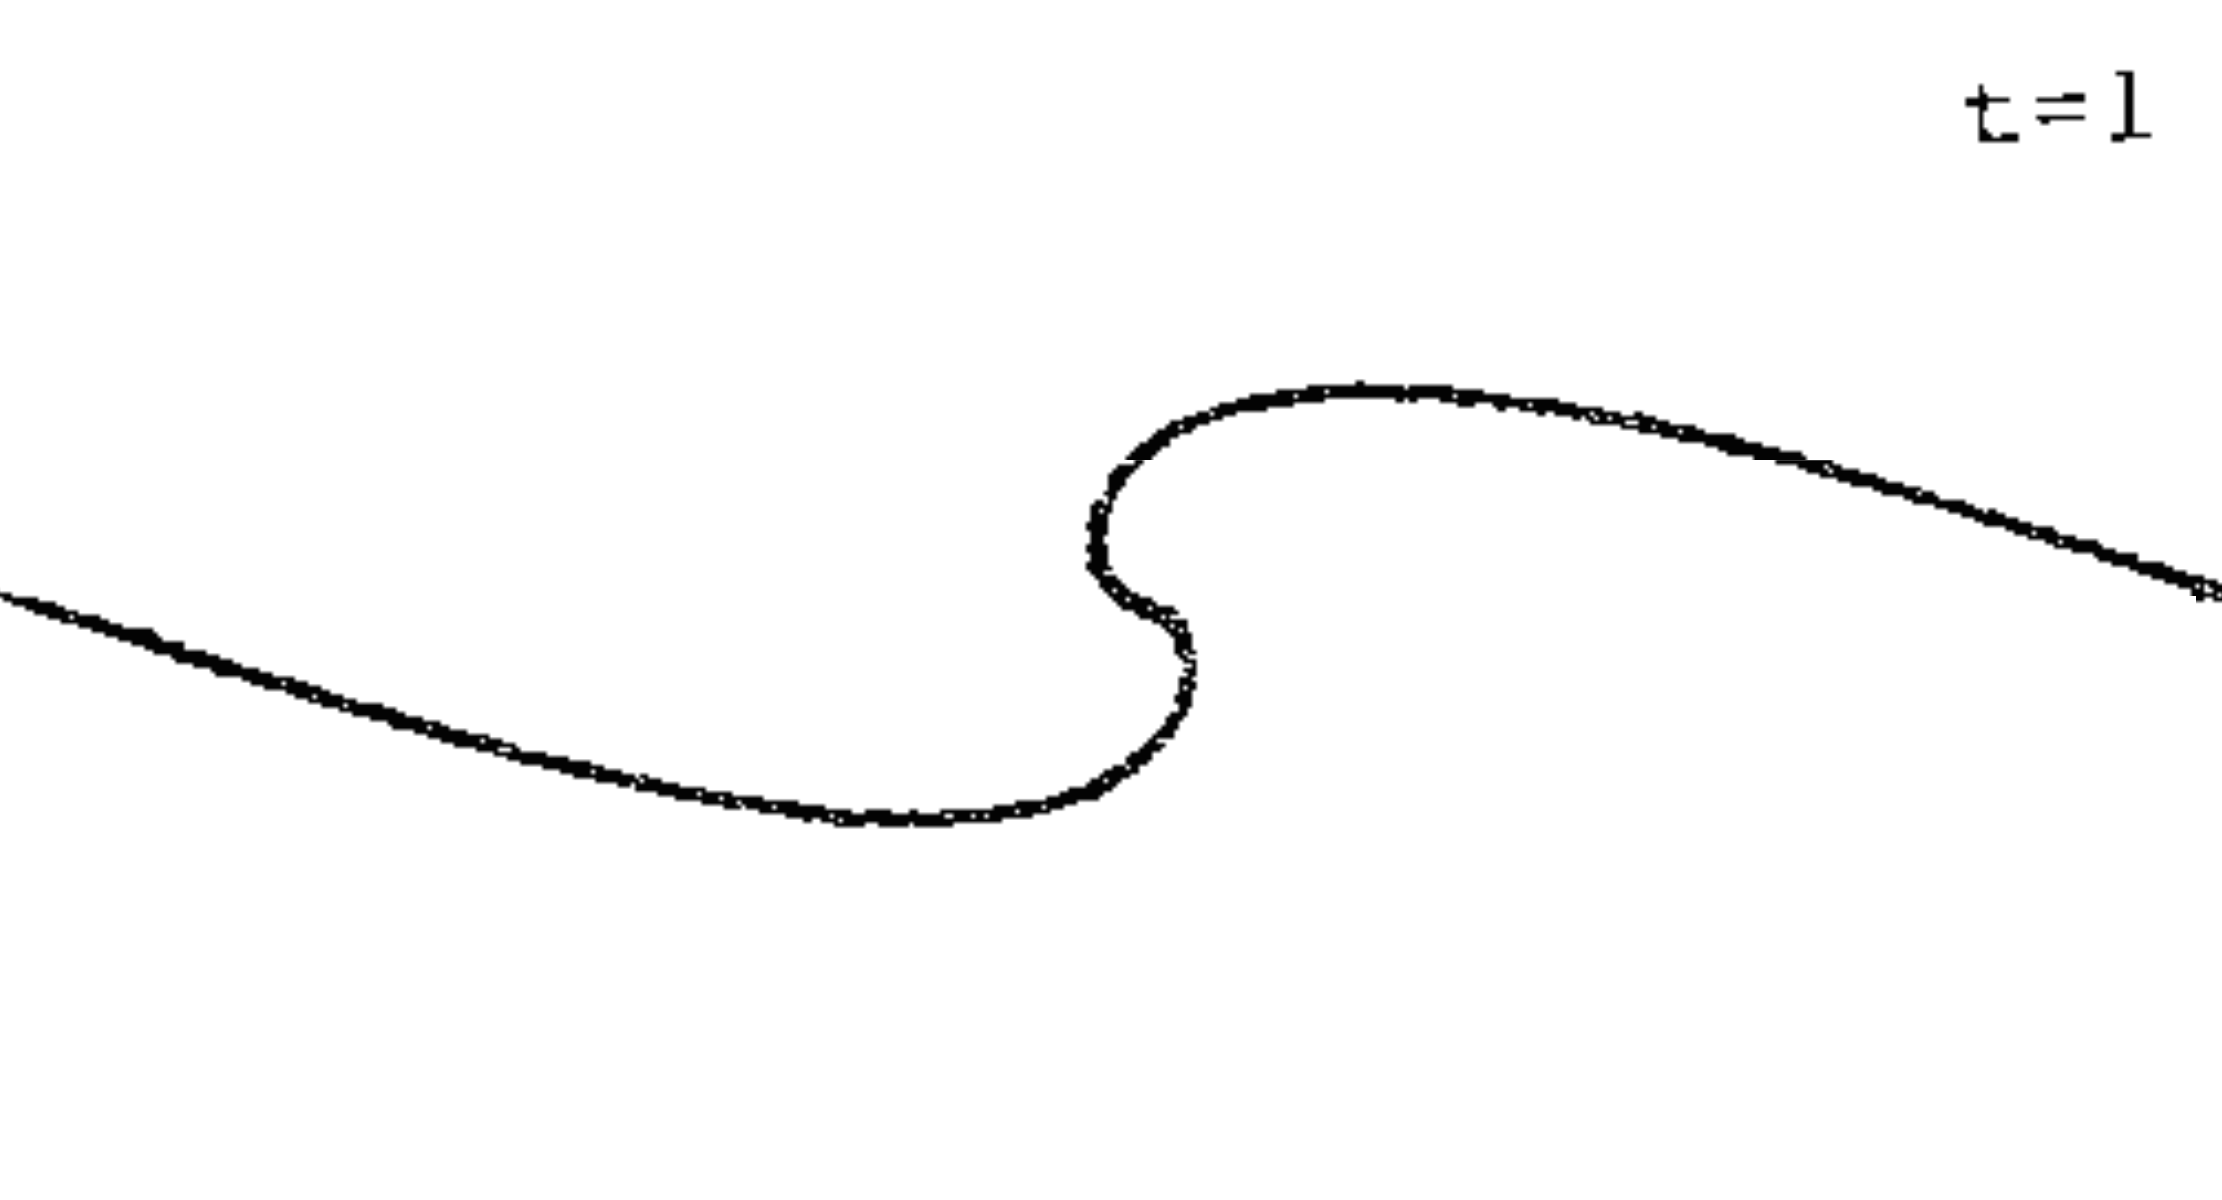
\includegraphics[width=1.5in,height=1.1in]{periodic21.png}

	\includegraphics[width=2in,height=1.33in]{K8.pdf}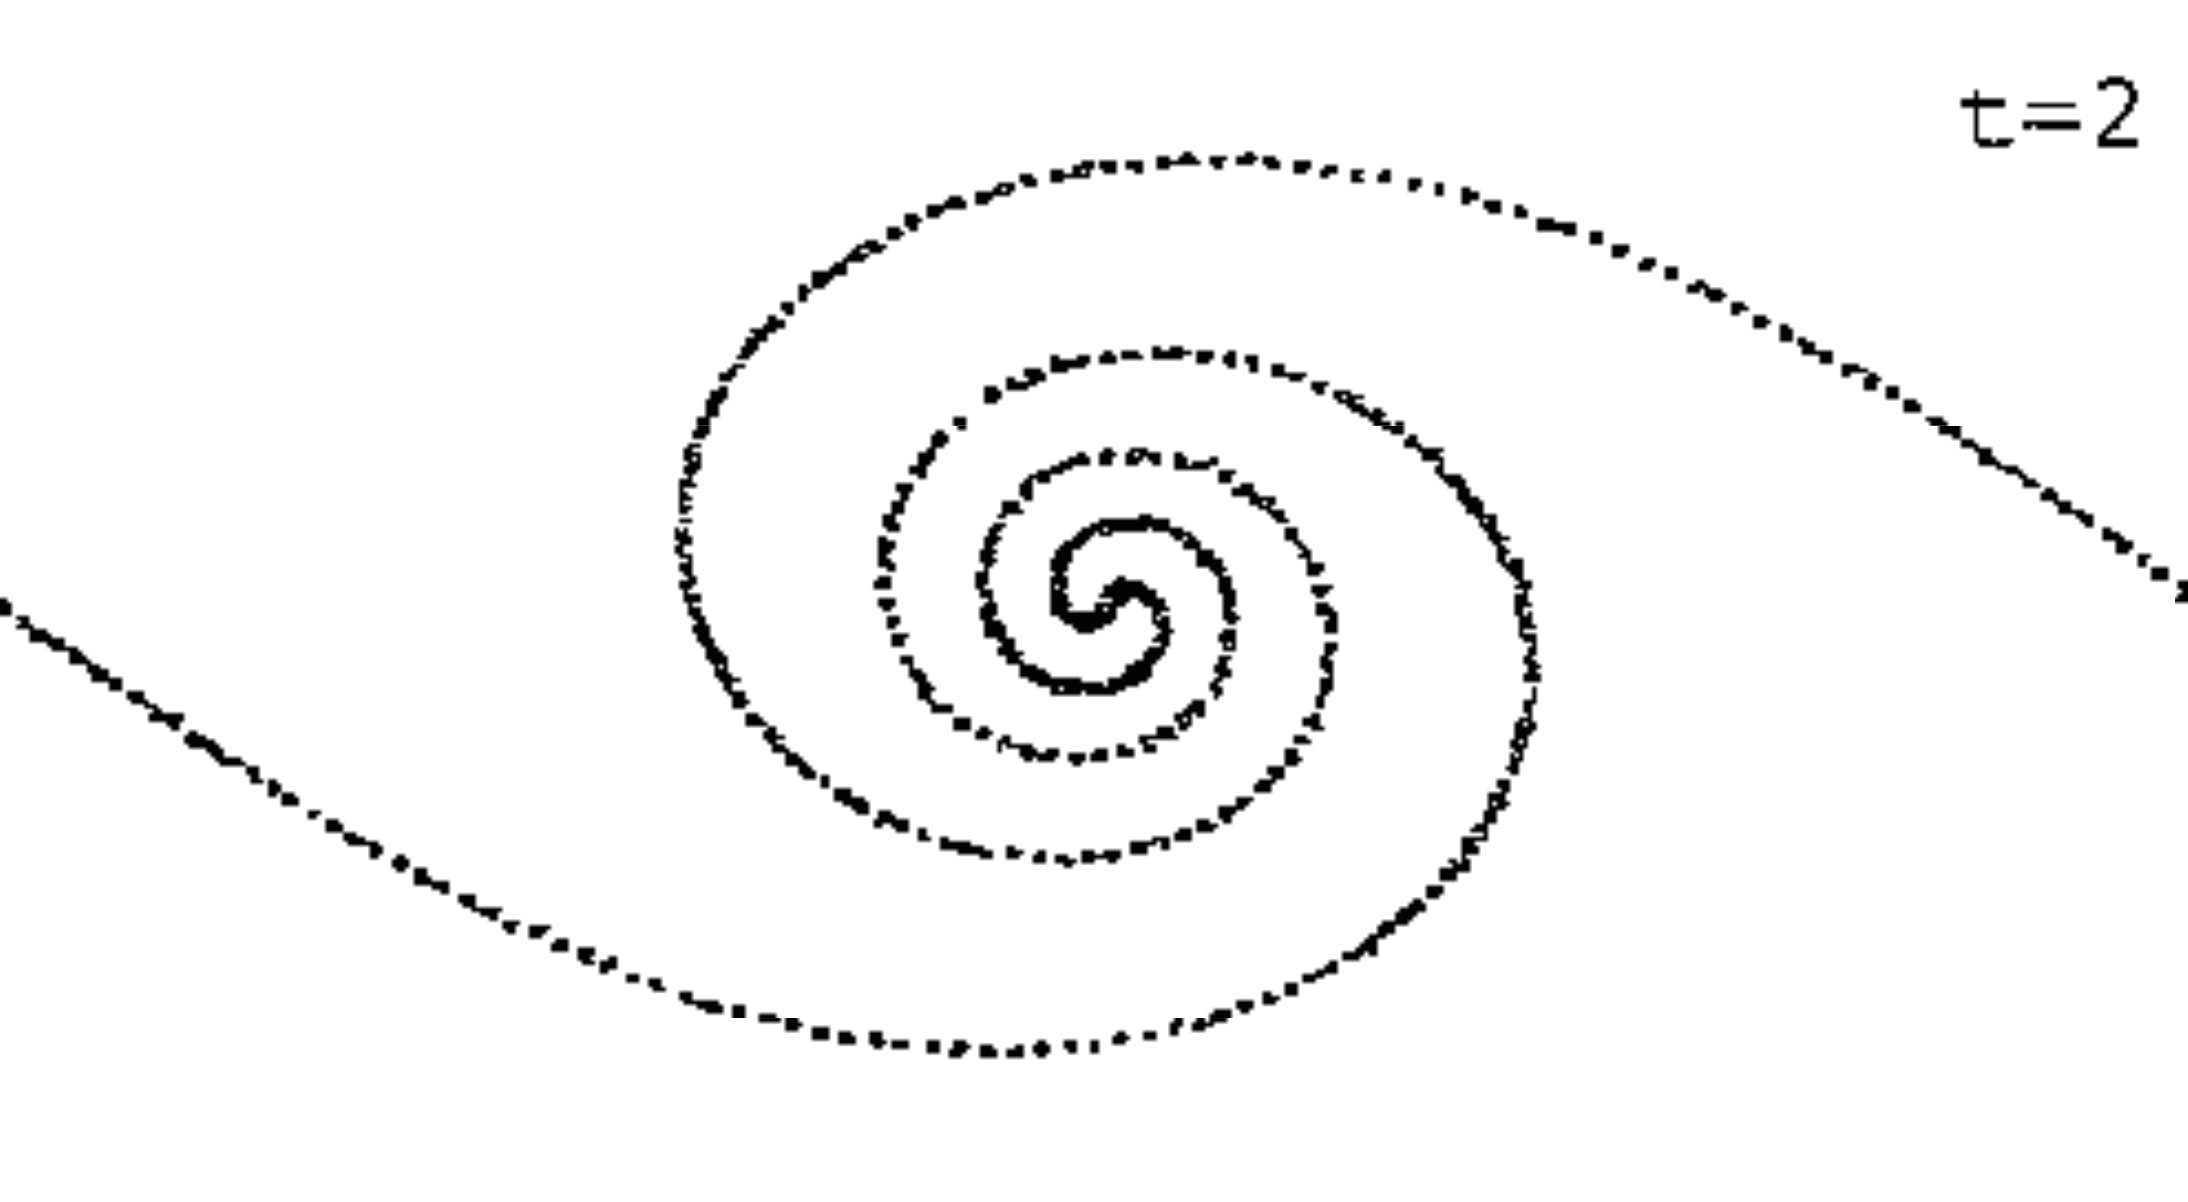
\includegraphics[width=1.5in,height=1.2in]{periodic22.png}

	\includegraphics[width=2in,height=1.33in]{K9.pdf}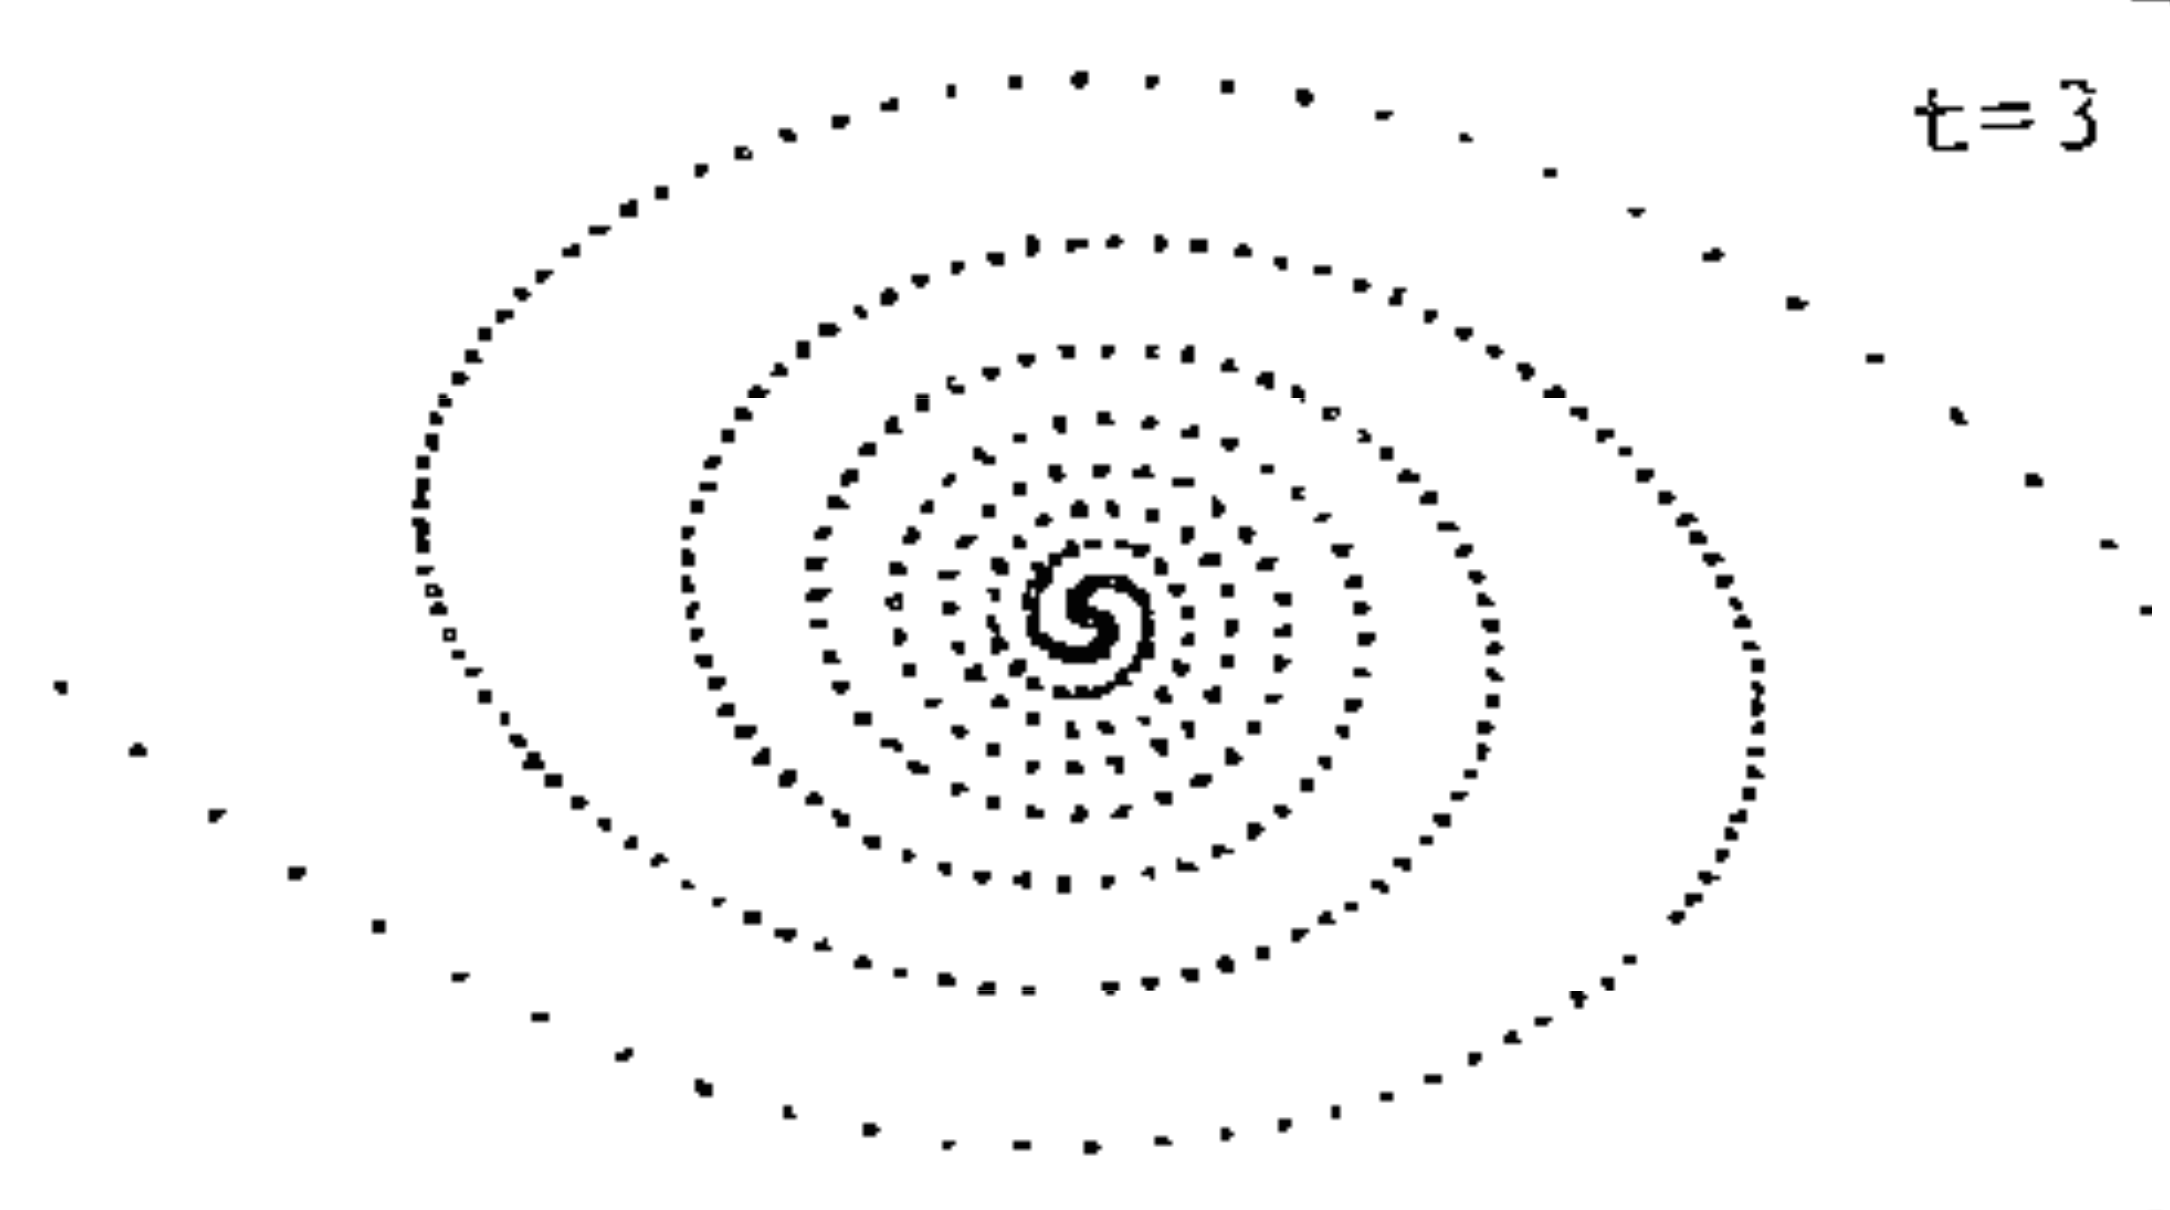
\includegraphics[width=1.5in,height=1.2in]{periodic23.png}

	\includegraphics[width=2in,height=1.33in]{K10.pdf}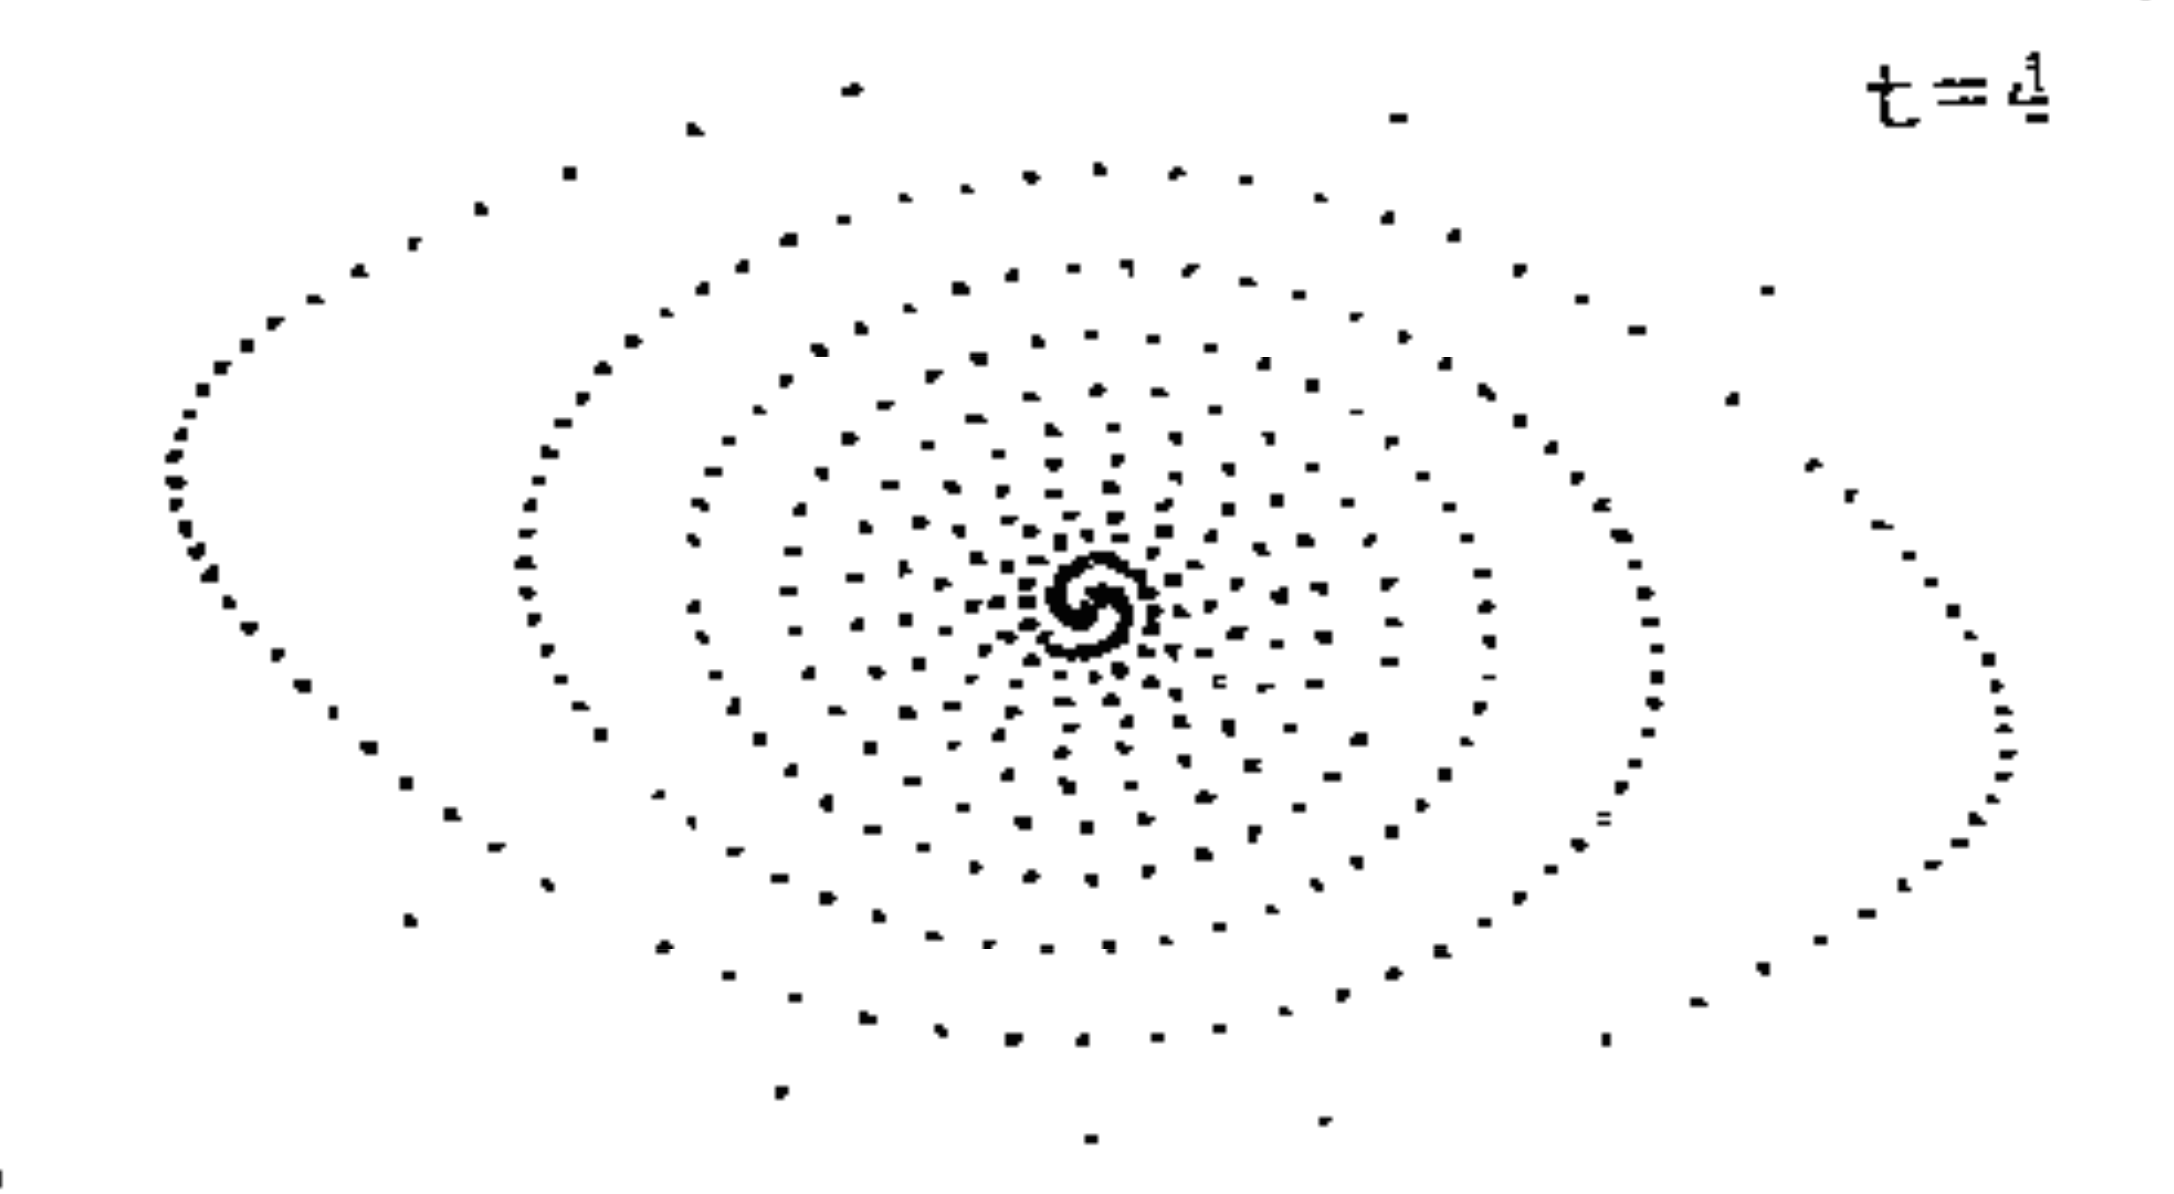
\includegraphics[width=1.5in,height=1.2in]{periodic24.png}
\end{center}
\caption{Periodic Vortex-Sheet Roll-up, with $N=400$, $\delta=0.25$ and $\Delta t=0.05$}
\end{figure}
\begin{figure}
\begin{center}
	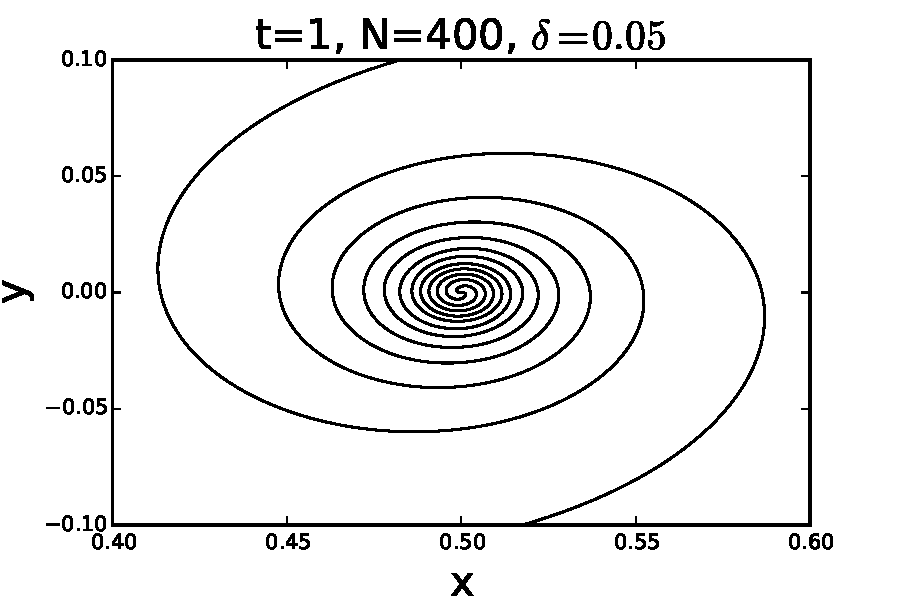
\includegraphics[width=2in,height=1.33in]{k11.pdf}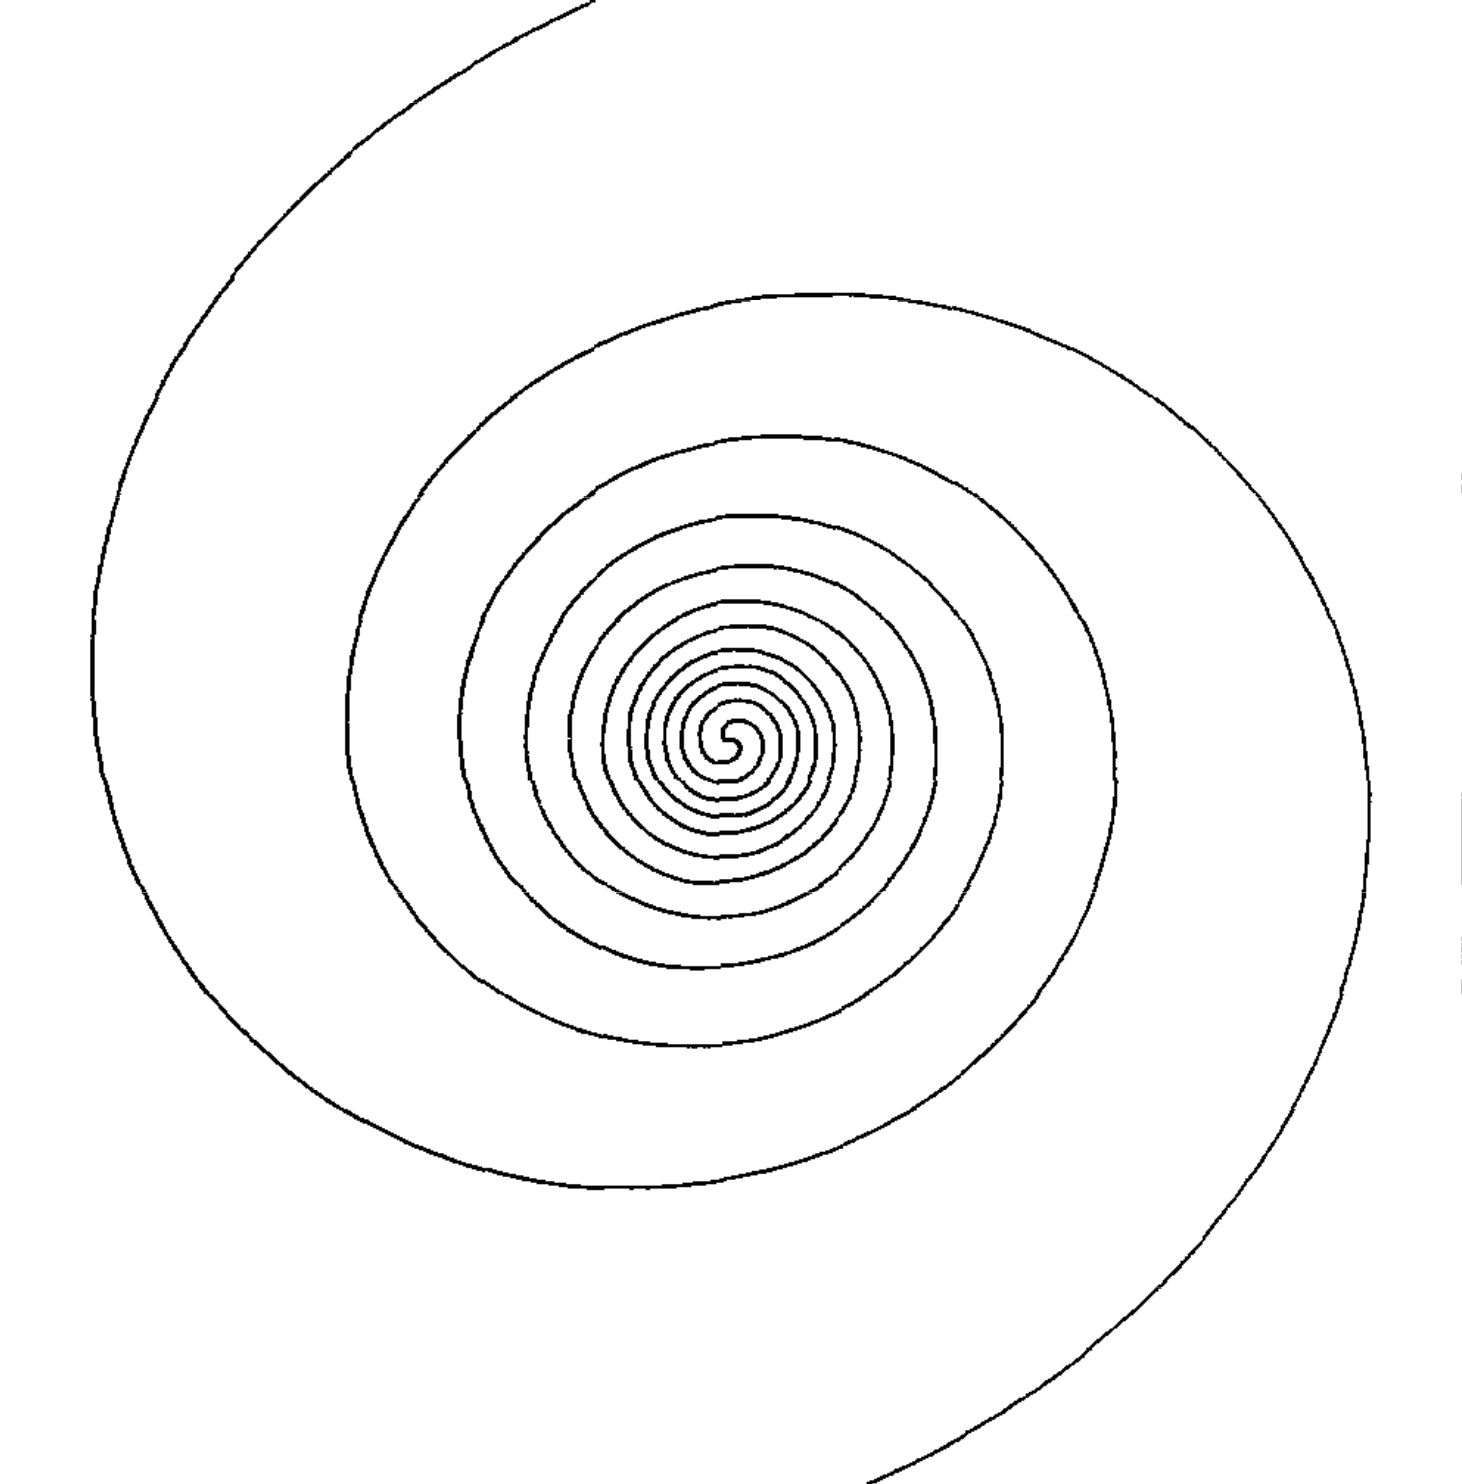
\includegraphics[width=1.5in,height=1.1in]{periodiccloseup.png}\\

\end{center}

\caption{Close-up view of the inner portion with $N=400$, $\delta=0.05$ and $\Delta t=0.01$}
\end{figure}
\clearpage

\begin{figure}[ht]
\centering
\begin{minipage}[b]{0.45\linewidth}
 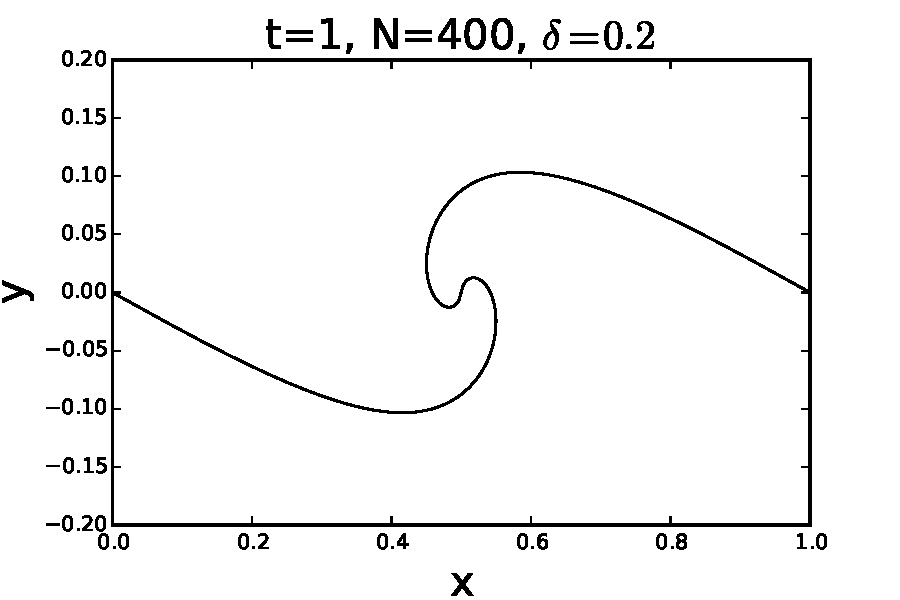
\includegraphics[width=2.7in,height=1.5in]{k12.pdf}
 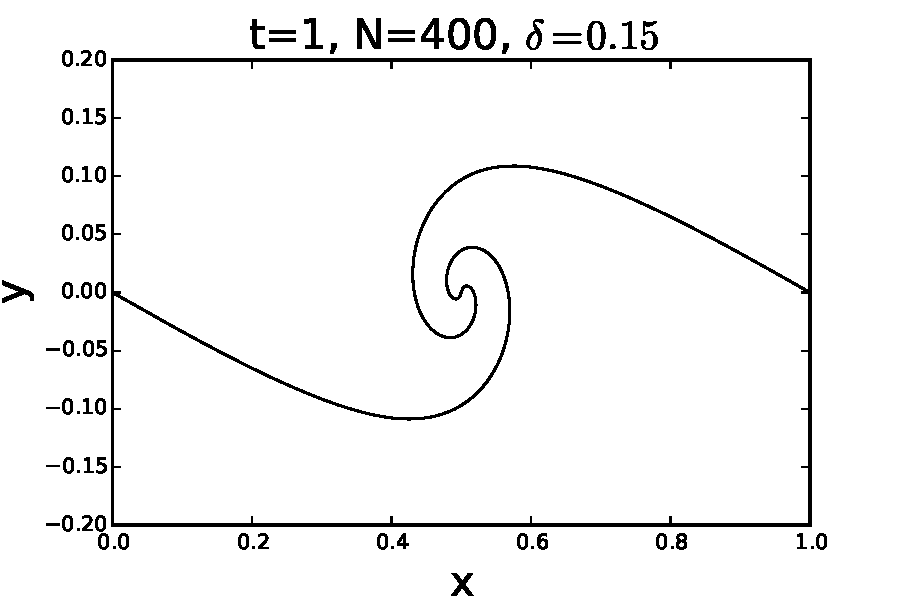
\includegraphics[width=2.7in,height=1.5in]{k13.pdf}
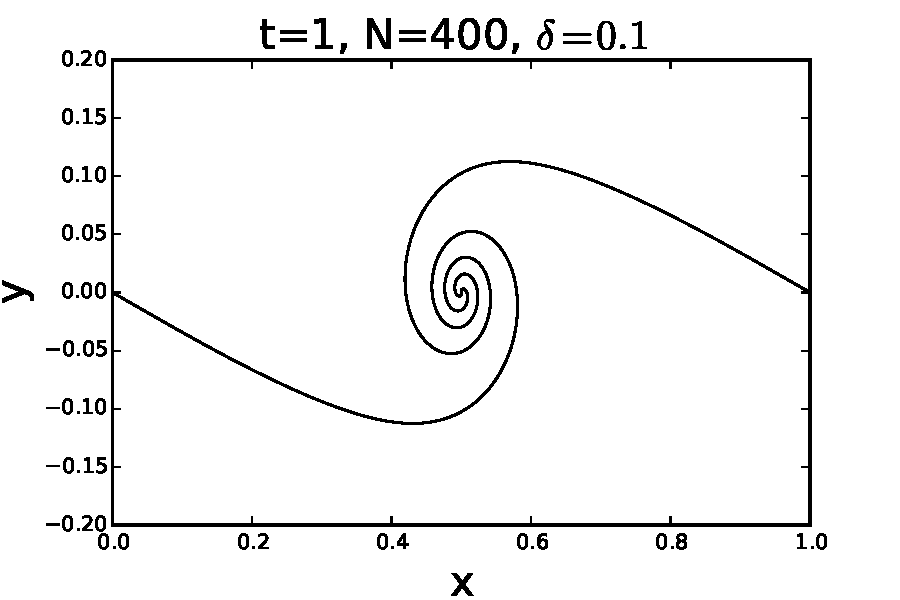
\includegraphics[width=2.7in,height=1.5in]{k14.pdf}
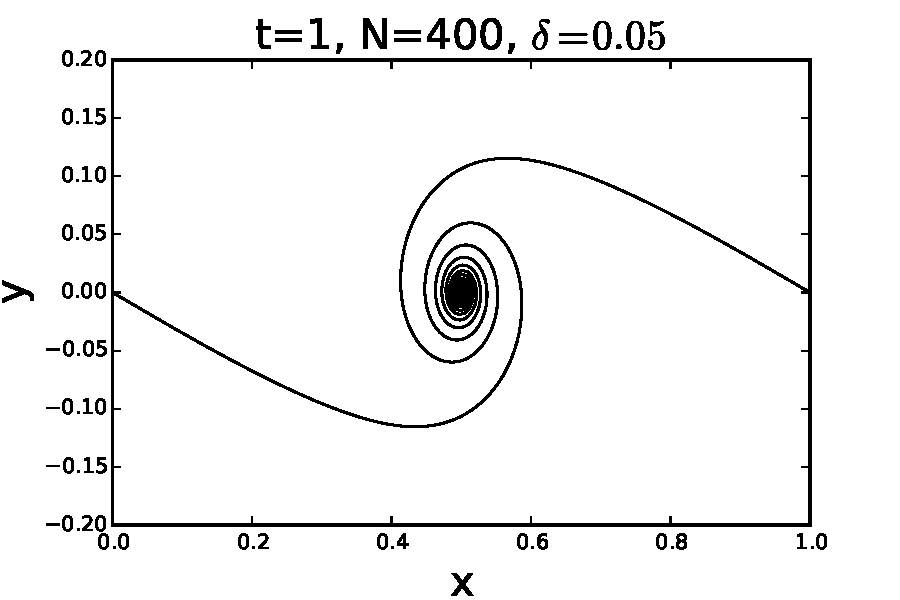
\includegraphics[width=2.7in,height=1.5in]{k15.pdf}
\label{fig:minipage2}
\end{minipage}
\quad
\begin{minipage}[b]{0.45\linewidth}
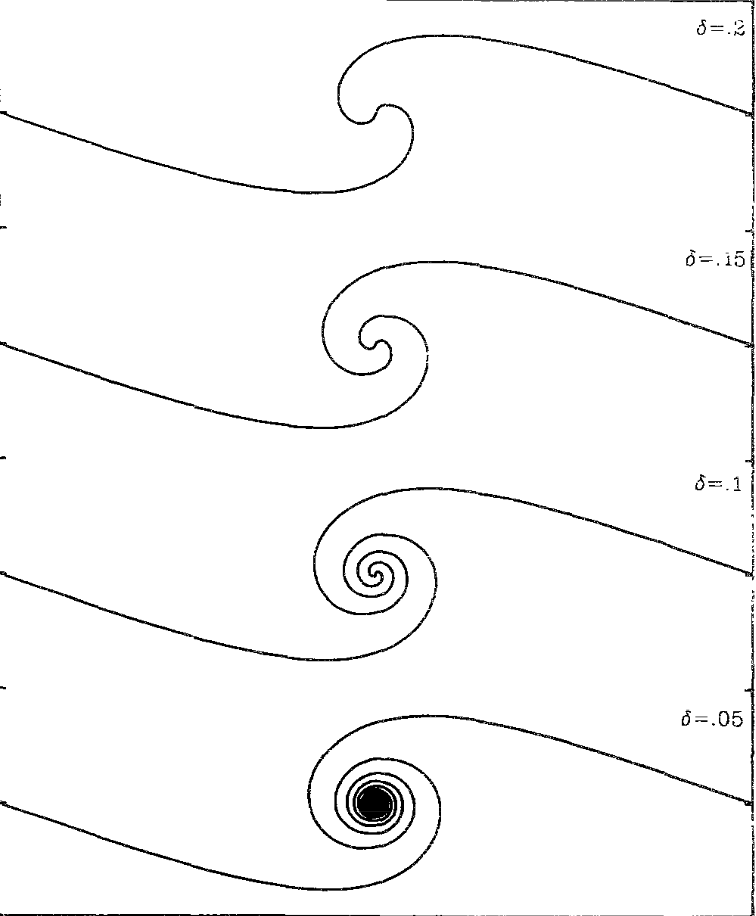
\includegraphics[width=2in,height=5.33in]{period.png}
\label{fig:minipage1}
\end{minipage}
\caption{Effect of decreasing $\delta$ in the $\delta$-equations at $t=1.0$ }
\end{figure}
\section{Trefftz Plane}
The initial conditions for the Trefftz plane is given by $z_j(0)=-\cos(\alpha_j)$.The circulation, $\Gamma$, for the trefftz plane is defined as $\Gamma(\alpha_j)=\sin(\alpha_j)$. In Figure 4 we show the early stage of the roll-up for $\Delta t=0.01$ and $\delta=0.05$ with $N=200$, where our results match the figures in $[2]$. We have plotted a trignometric interpolating polynomial in the variable $\alpha$, the coefficients of the polynomial where calculated using a discrete cosine transform of the $z_j$ values obtained after integrating. 
\begin{figure}
\begin{center}
	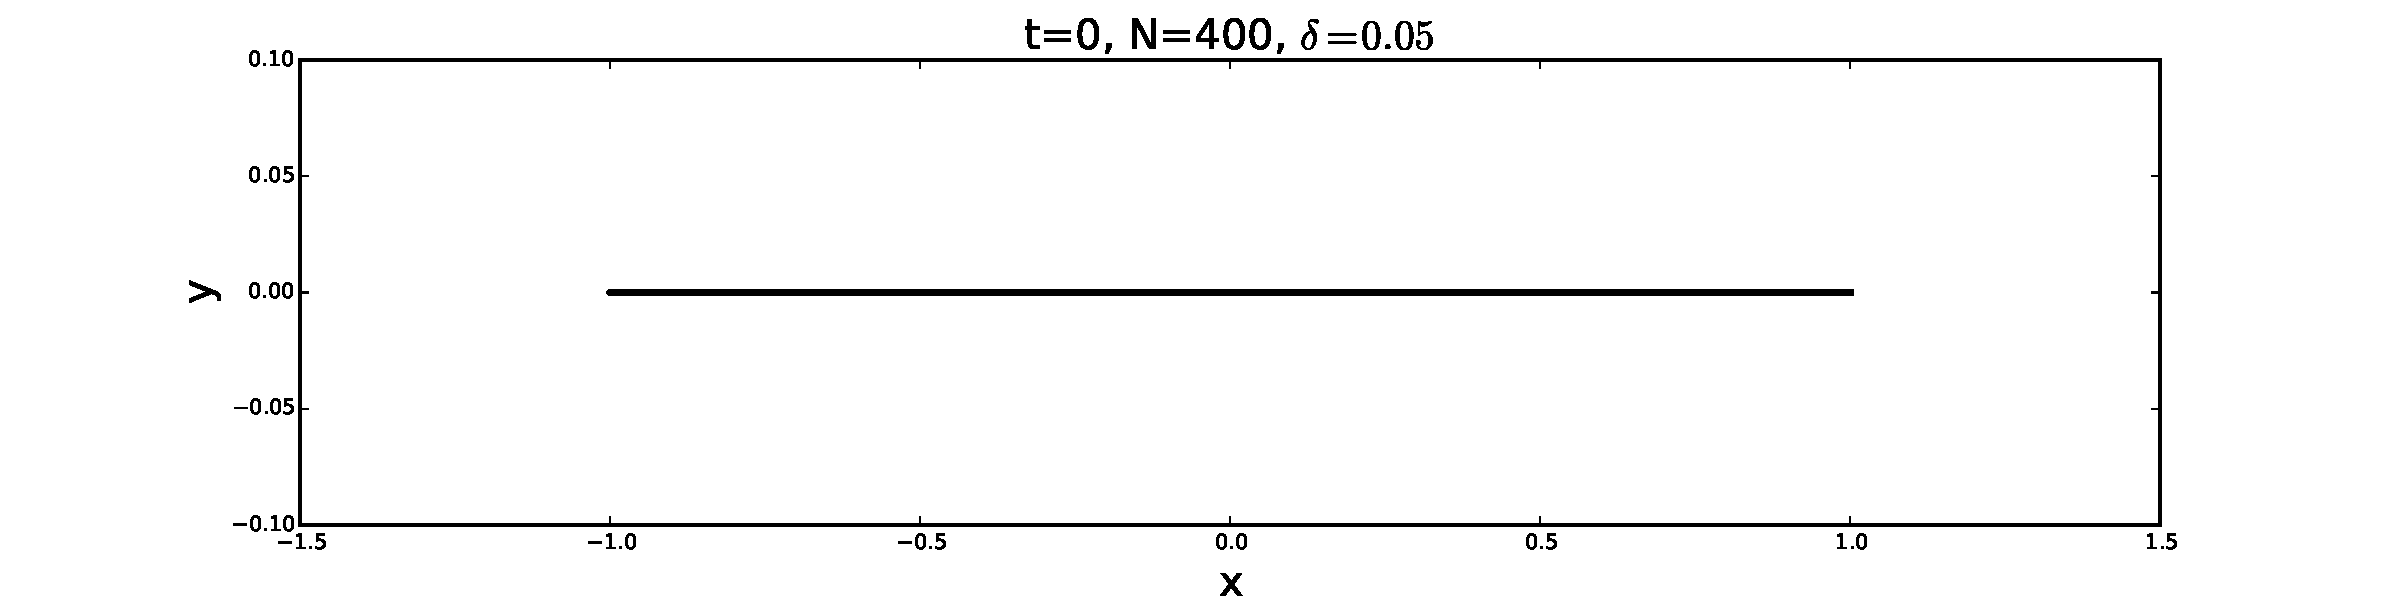
\includegraphics[width=3in,height=1.33in]{tr1.pdf} \raisebox{0.9\height}{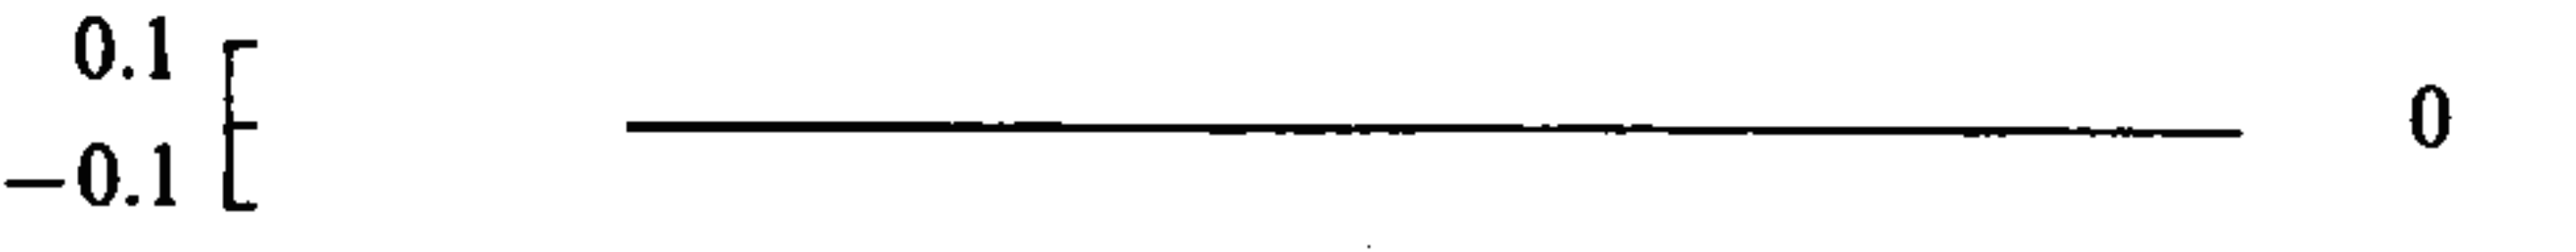
\includegraphics[width=2.5in,height=0.4in]{Tref0.png}}
	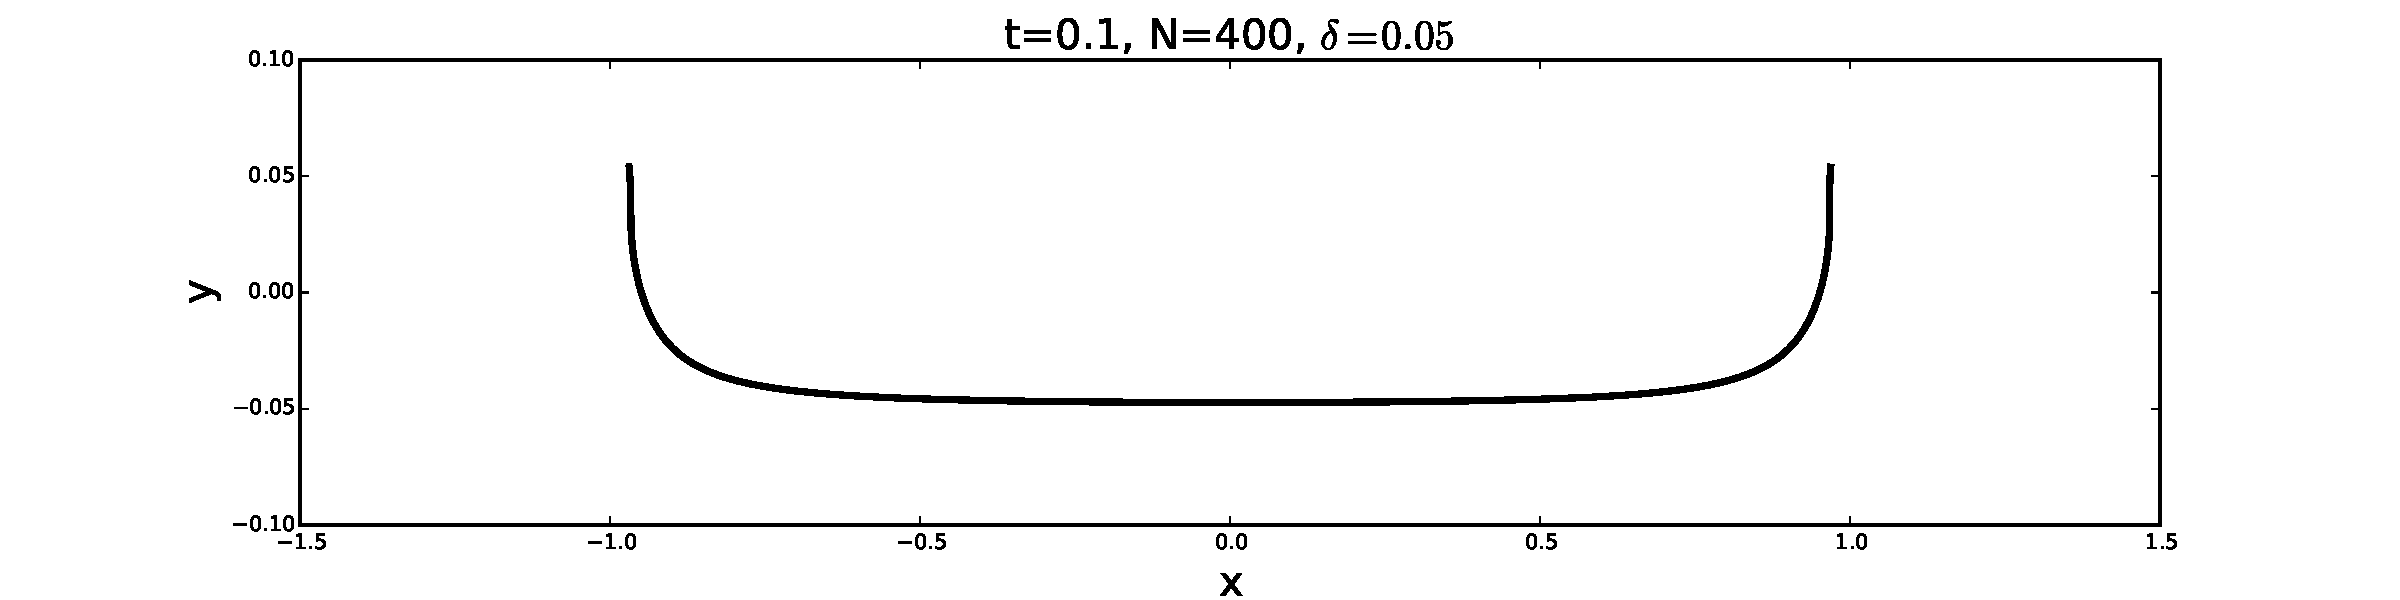
\includegraphics[width=3in,height=1.33in]{tr2.pdf}\raisebox{1\height}{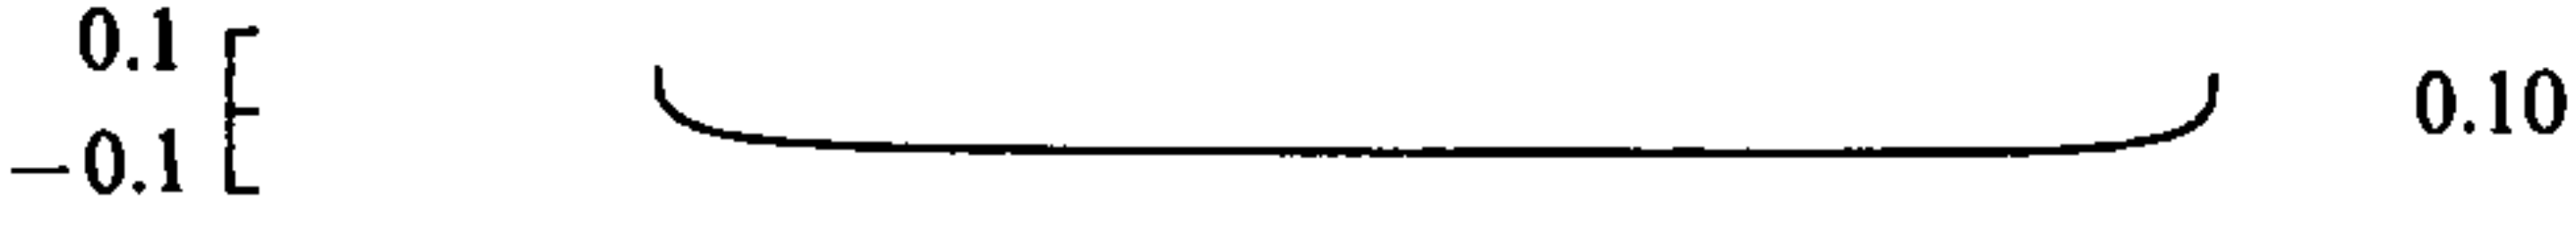
\includegraphics[width=2.5in,height=0.4in]{Tref1.png}}
	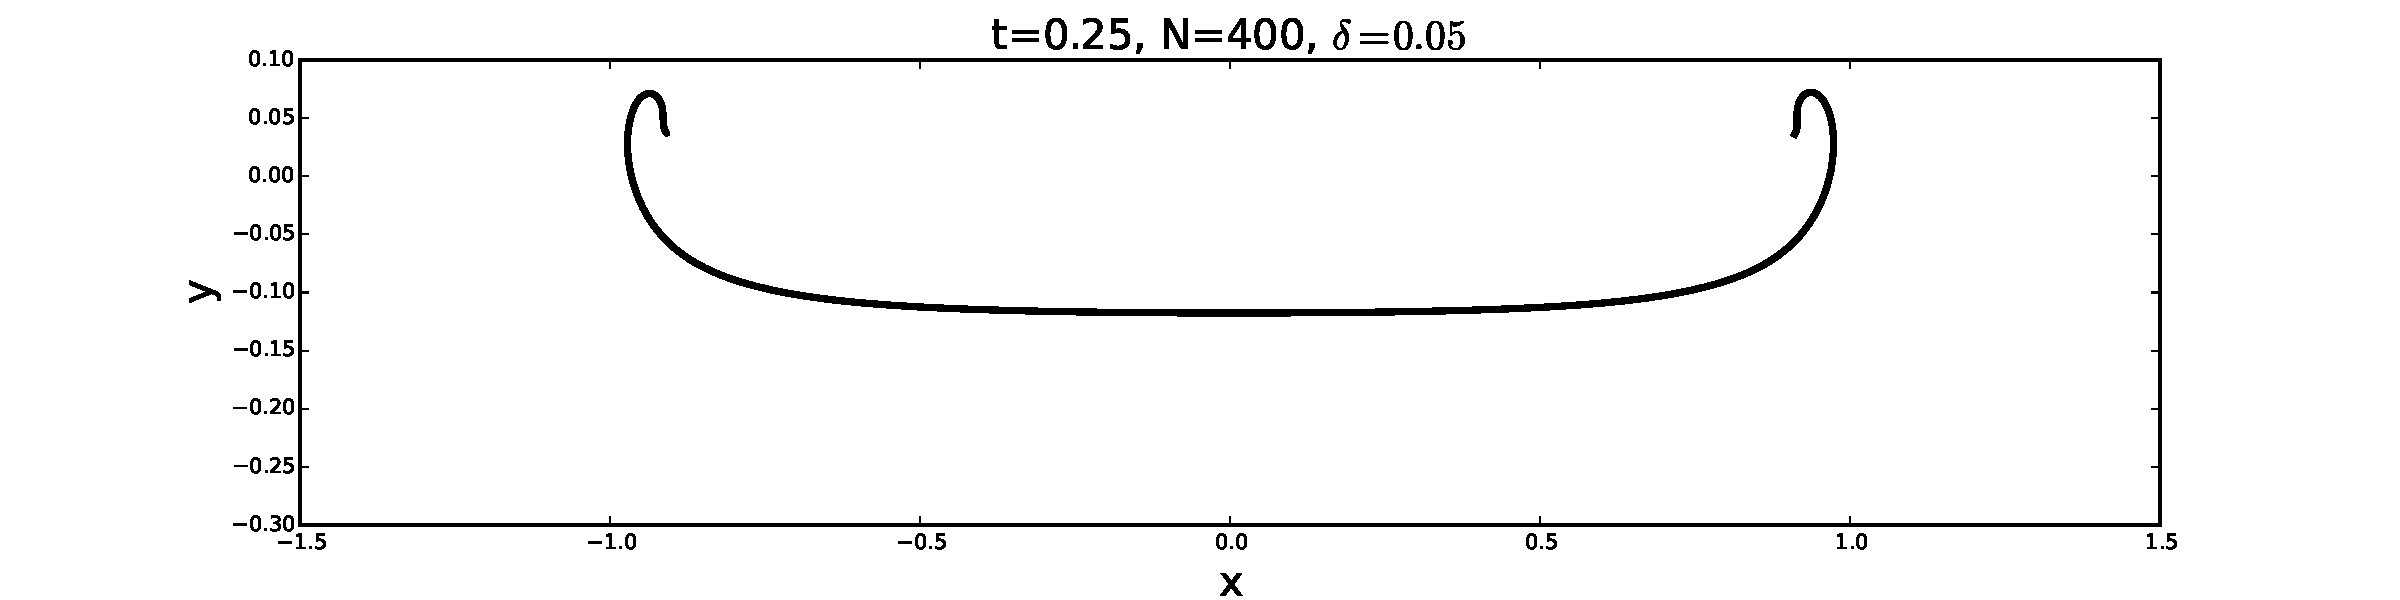
\includegraphics[width=3in,height=1.33in]{tr3.pdf}\raisebox{0.9\height}{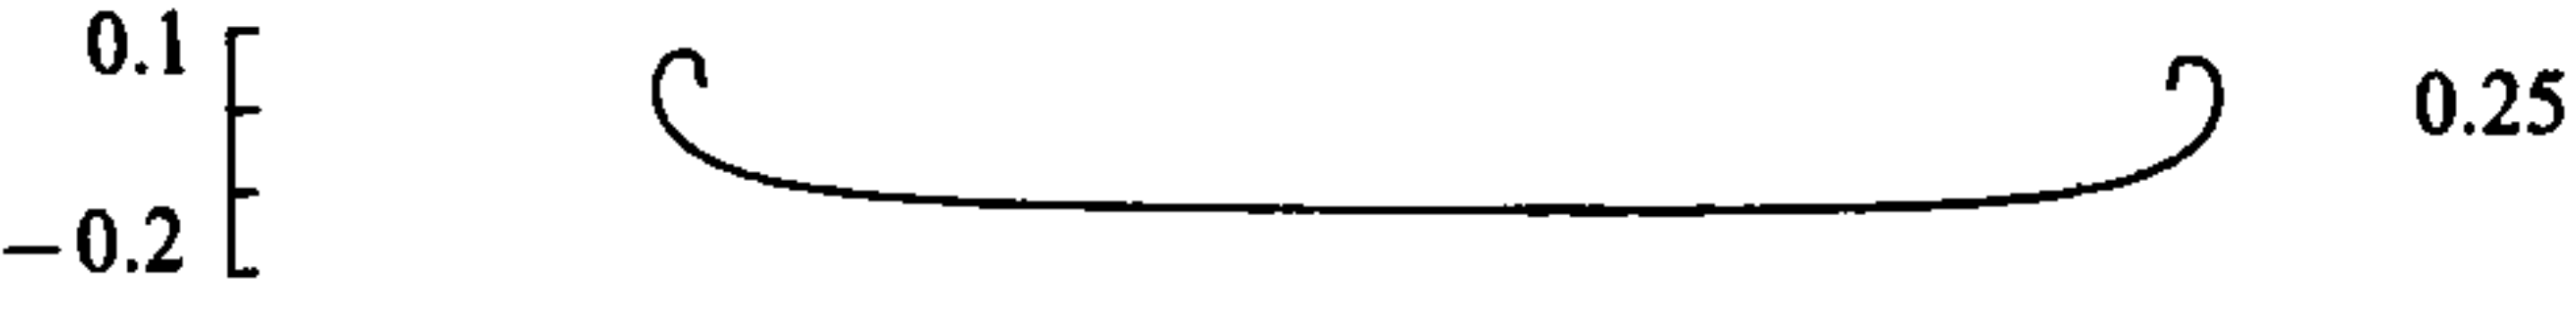
\includegraphics[width=2.5in,height=0.45in]{Tref2.png}}

	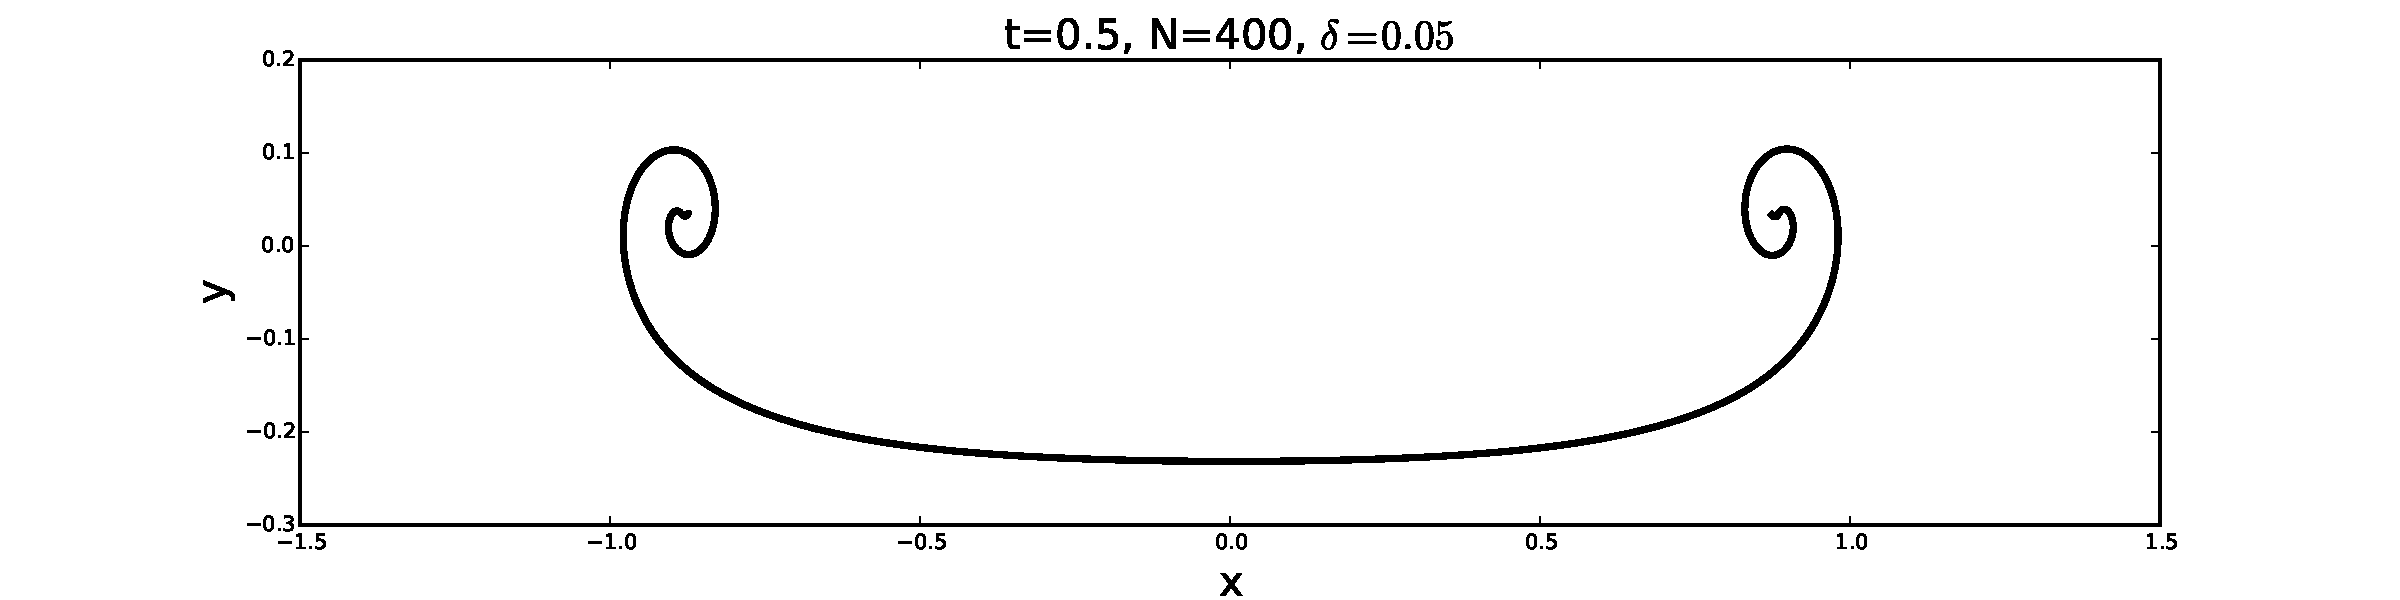
\includegraphics[width=3in,height=1.33in]{tr4.pdf}\raisebox{0.75\height}{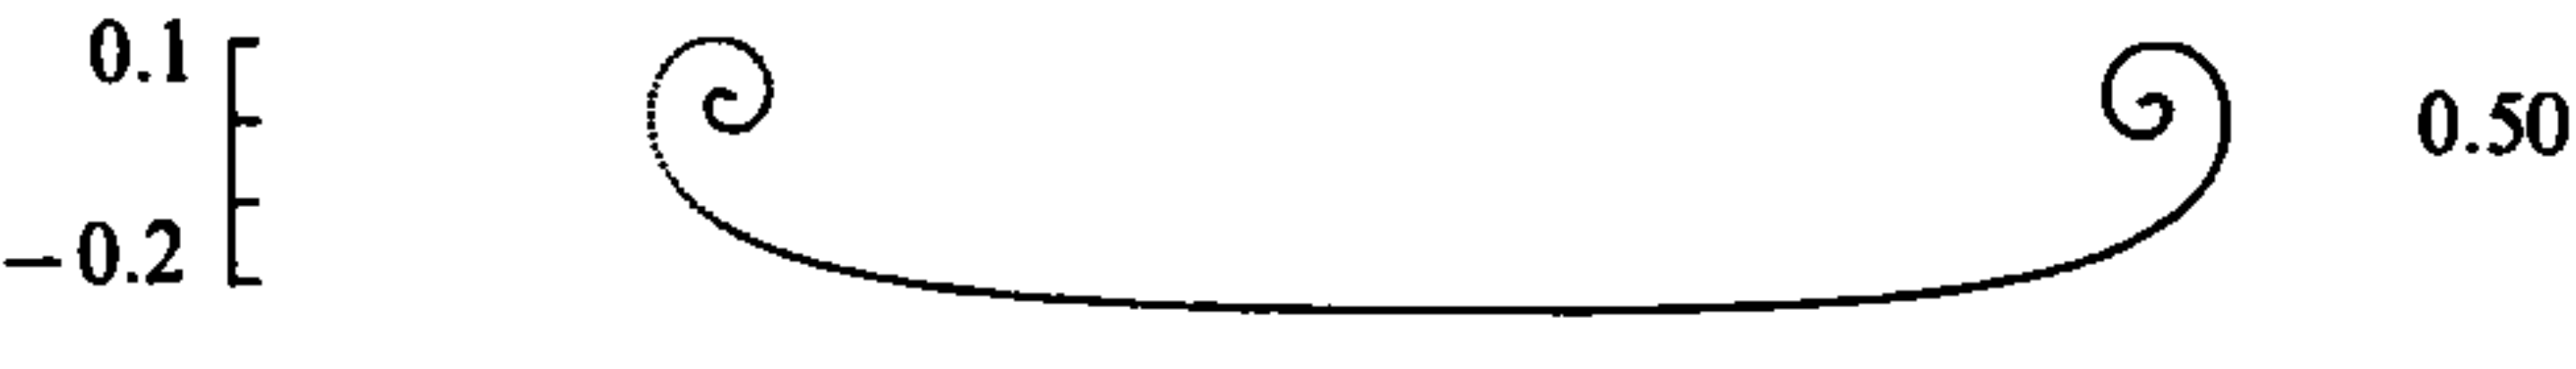
\includegraphics[width=2.5in,height=0.5in]{Tref3.png}}

	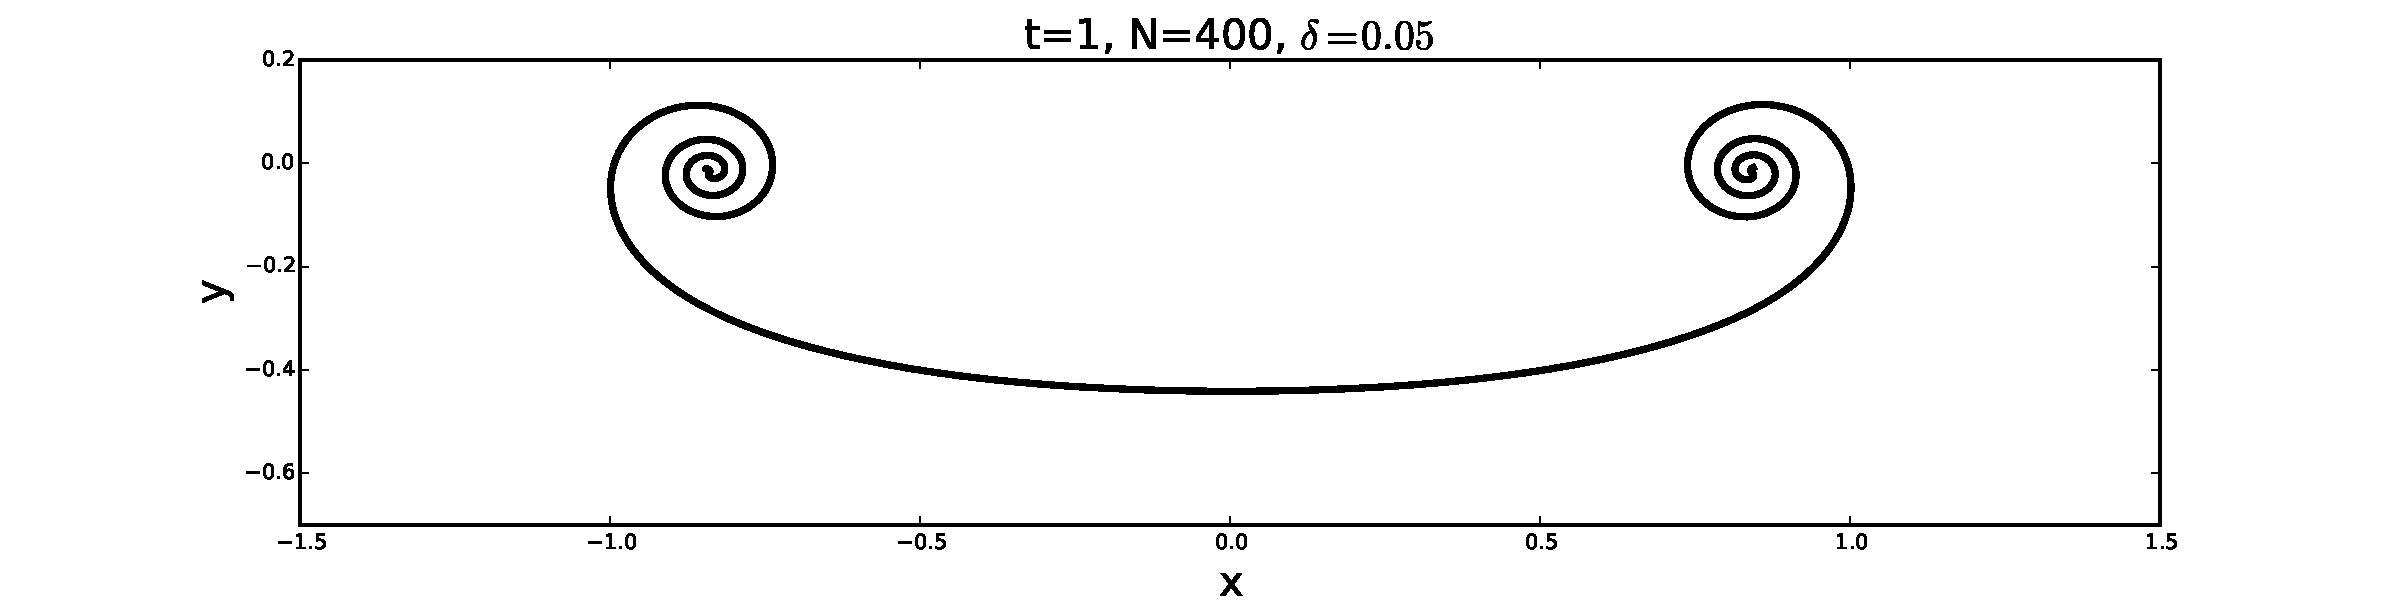
\includegraphics[width=3in,height=1.33in]{tr5.pdf}\raisebox{0.6\height}{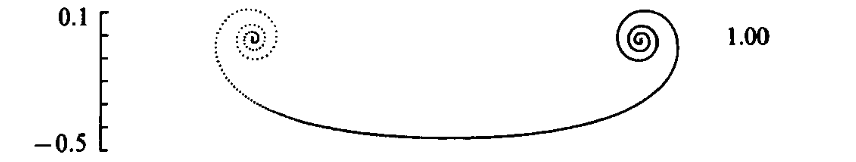
\includegraphics[width=2.5in,height=0.7in]{Tref4.png}}



	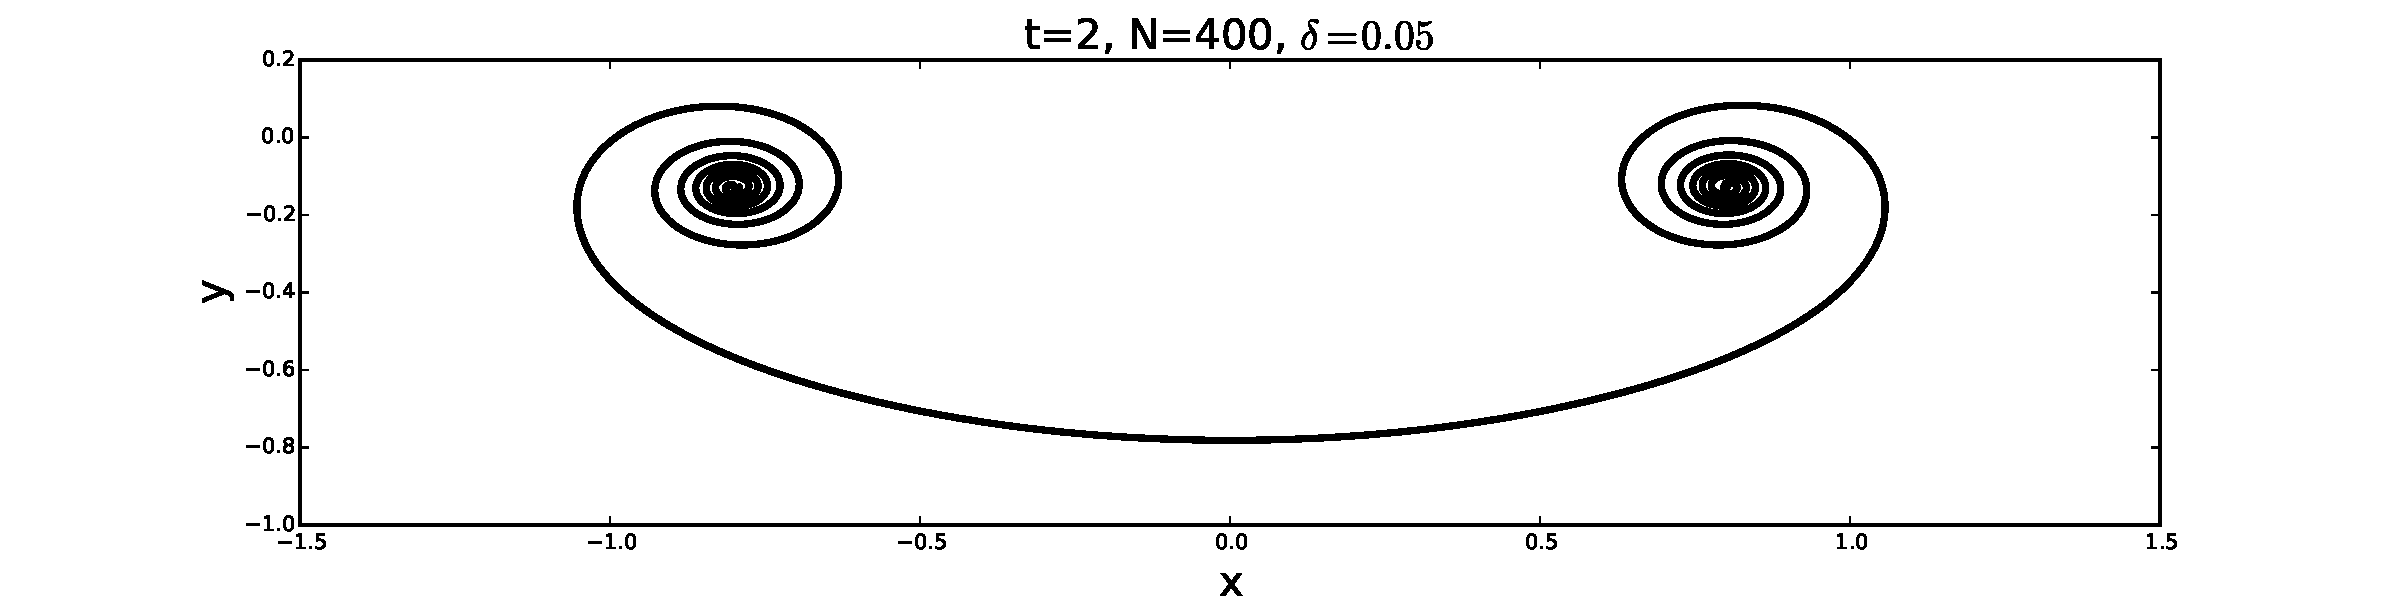
\includegraphics[width=3in,height=1.33in]{tr6.pdf}\raisebox{0.6\height}{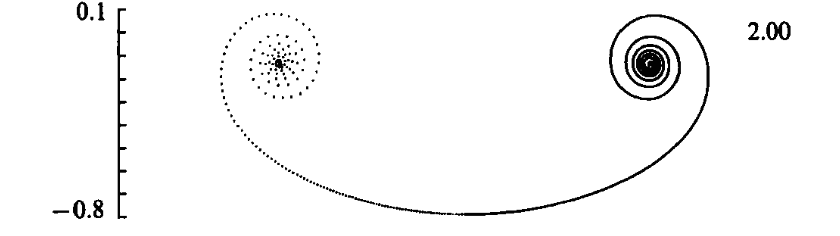
\includegraphics[width=2.5in,height=0.7in]{Tref5.png}}


	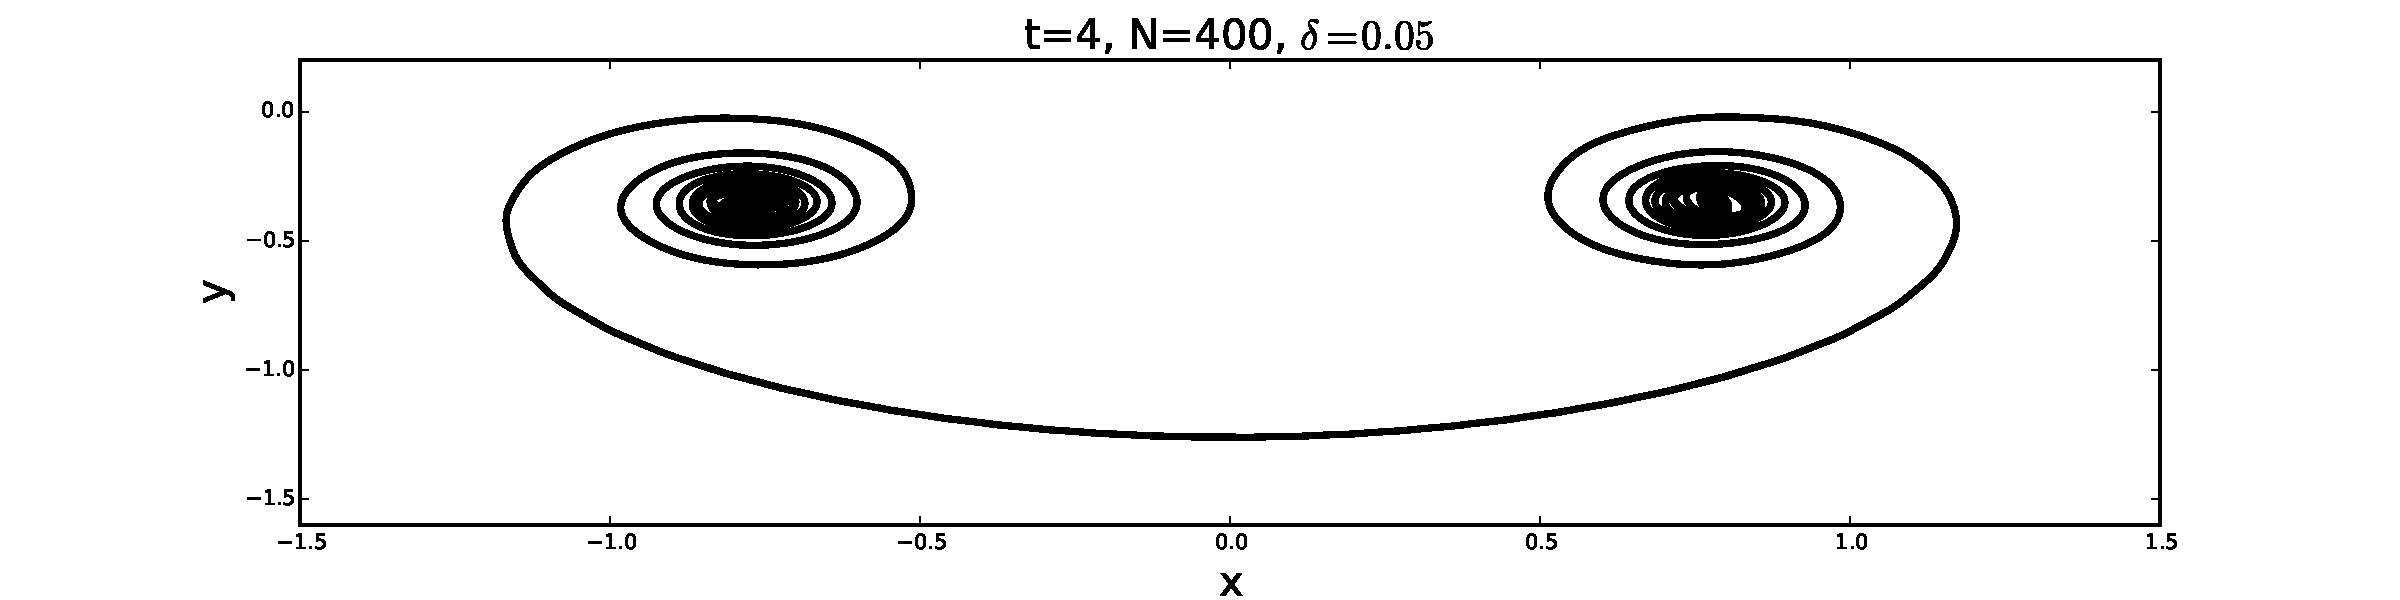
\includegraphics[width=3in,height=1.33in]{tr7.pdf}\raisebox{0.6\height}{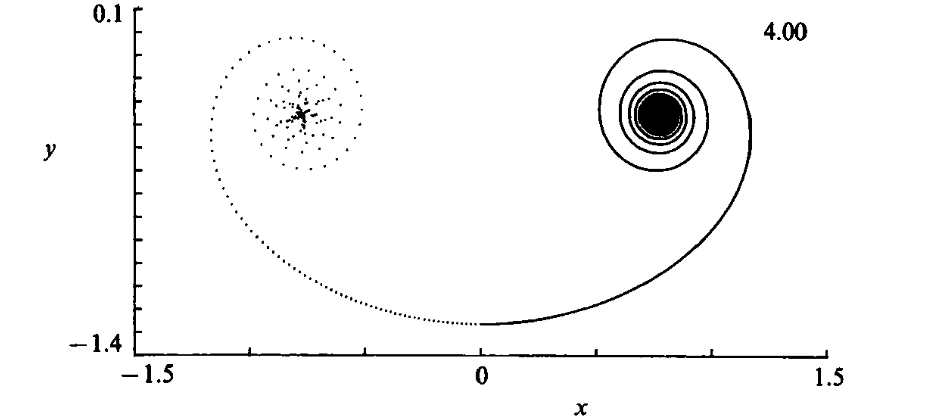
\includegraphics[width=2.5in,height=0.7in]{Tref6.png}}
\caption{Early stage of the roll-up in the Trefftz plane, with $N=200$, $\delta=0.05$ and $\Delta t=0.01$}
\end{center}
\end{figure}
\clearpage

\section{Elliptically Loaded Wing}
The initial conditions for the elliptically loaded wing is similarly defined as $z_j(0)=-\cos(\alpha_j)$.
Now, the circulation, $\Gamma$ is defined as follows:
\\1. For $1\ge{|x(\alpha_j)|}\ge{0.7}$, $\Gamma(\alpha_j)=\sin(\alpha_j)$
\\2. For $0.3\ge{|x(\alpha_j)|}\ge{0.0}$, and for $0.7\ge{|x(\alpha_j)|}\ge{0.3}$ , $\Gamma$ is a cubic polynomial in the variable $|x|$ .The coefficinets are chosen such that $\Gamma$ and $\Gamma'$ are continuous and that there is a global maximum at $|x|=0.3$, with $\Gamma=2.0$, and a local minimum at $|x|=0$ with $\Gamma=1.4$. 
\subsection{Early and Middle stages}
In figure 5 below we show the early stages of the roll-up for $\Delta t=0.1$ and $\delta=0.02$ with $N=200$, but to obtain the middle and late stages we encounter computational difficulties as there is excessive stretching at the end points causing the curves to intersect. To overcome this issue we employ a point insertion technique at each time step. First we set a mesh-parameter $\epsilon$, and then we demand that if $|z_j-z_j+1|\ge{\epsilon}$ then we insert a new point. The new point is computed using a cubic spline in the variable $\alpha$ , defined uniquely by the four neighbouring points. The inserted point is $\alpha=(\alpha_j + \alpha_{j+1})/2$. 

















\begin{figure}
\begin{center}
	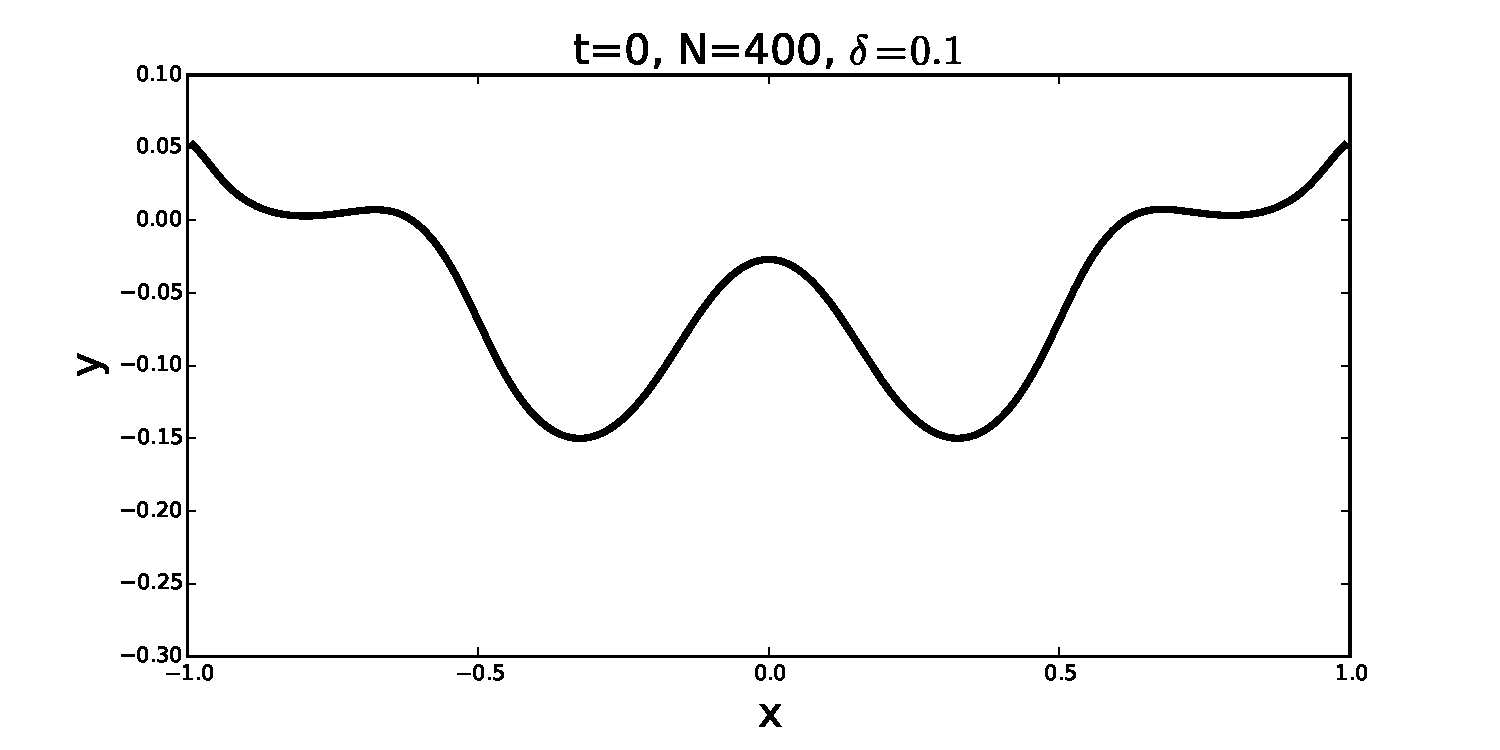
\includegraphics[width=3in,height=1.33in]{FU1.pdf}\raisebox{0.9\height}{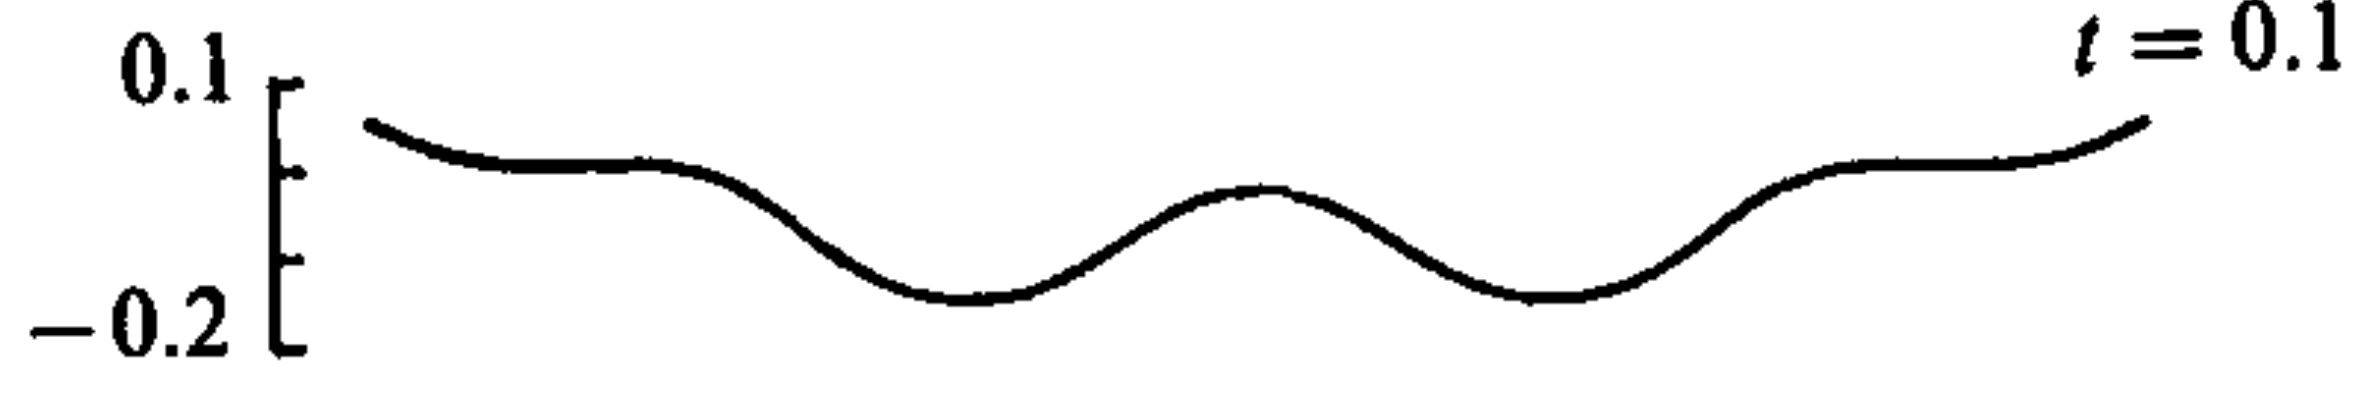
\includegraphics[width=2in,height=0.5in]{fuse1.png}}

	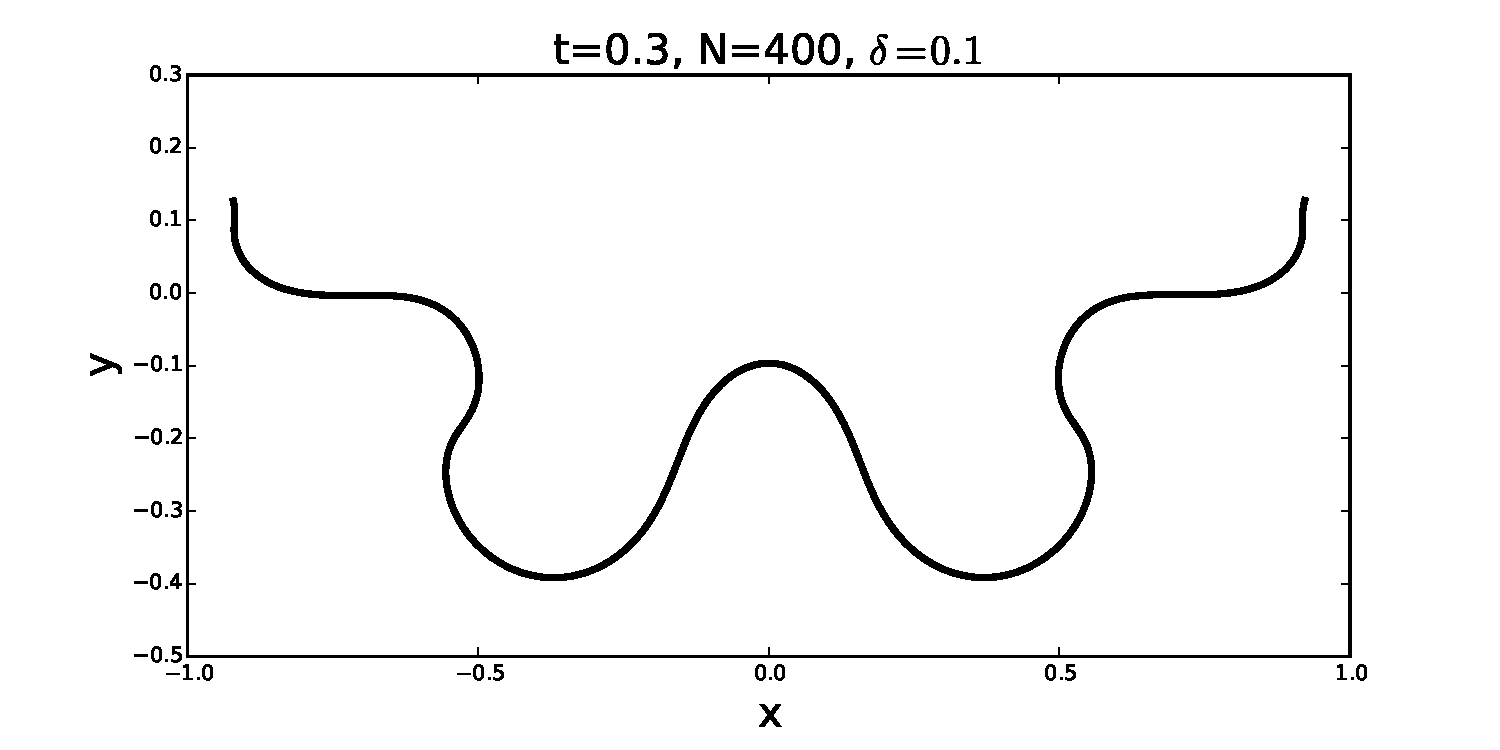
\includegraphics[width=3in,height=1.33in]{FU2.pdf}\raisebox{0.53\height}{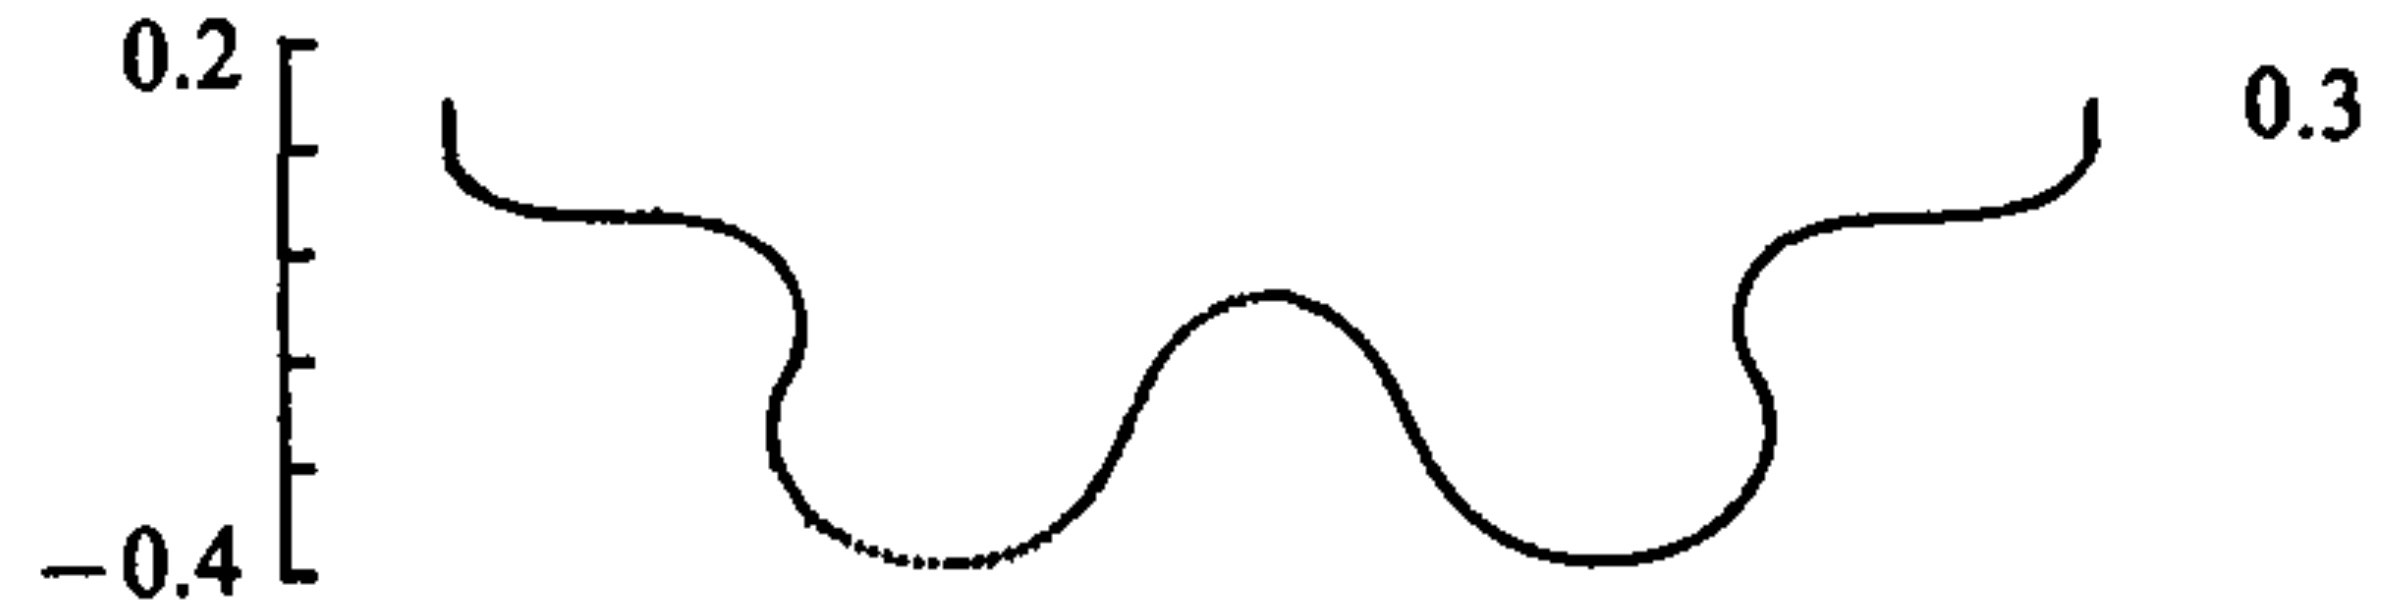
\includegraphics[width=2in,height=0.7in]{fuse2.png}}

	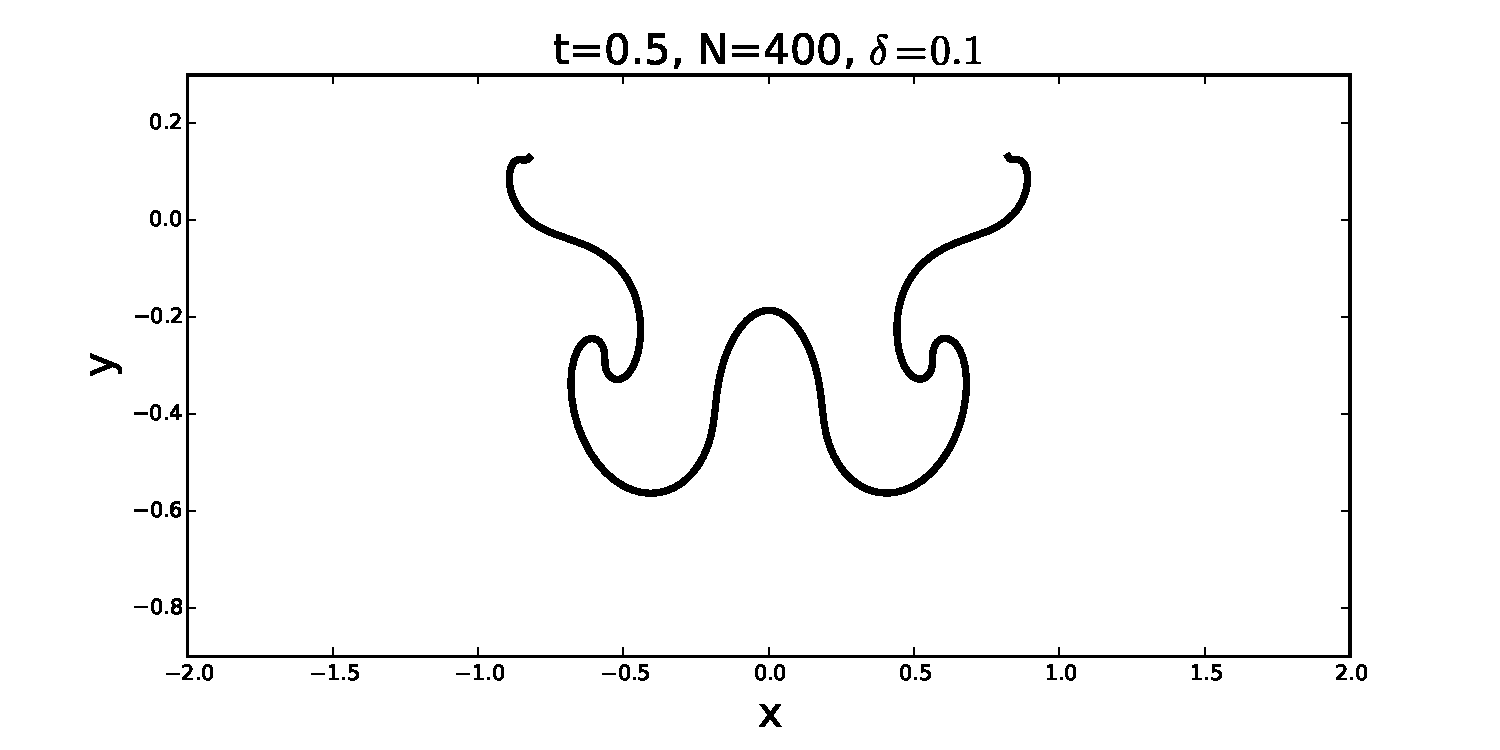
\includegraphics[width=3in,height=1.33in]{FU3.pdf}\raisebox{0.15\height}{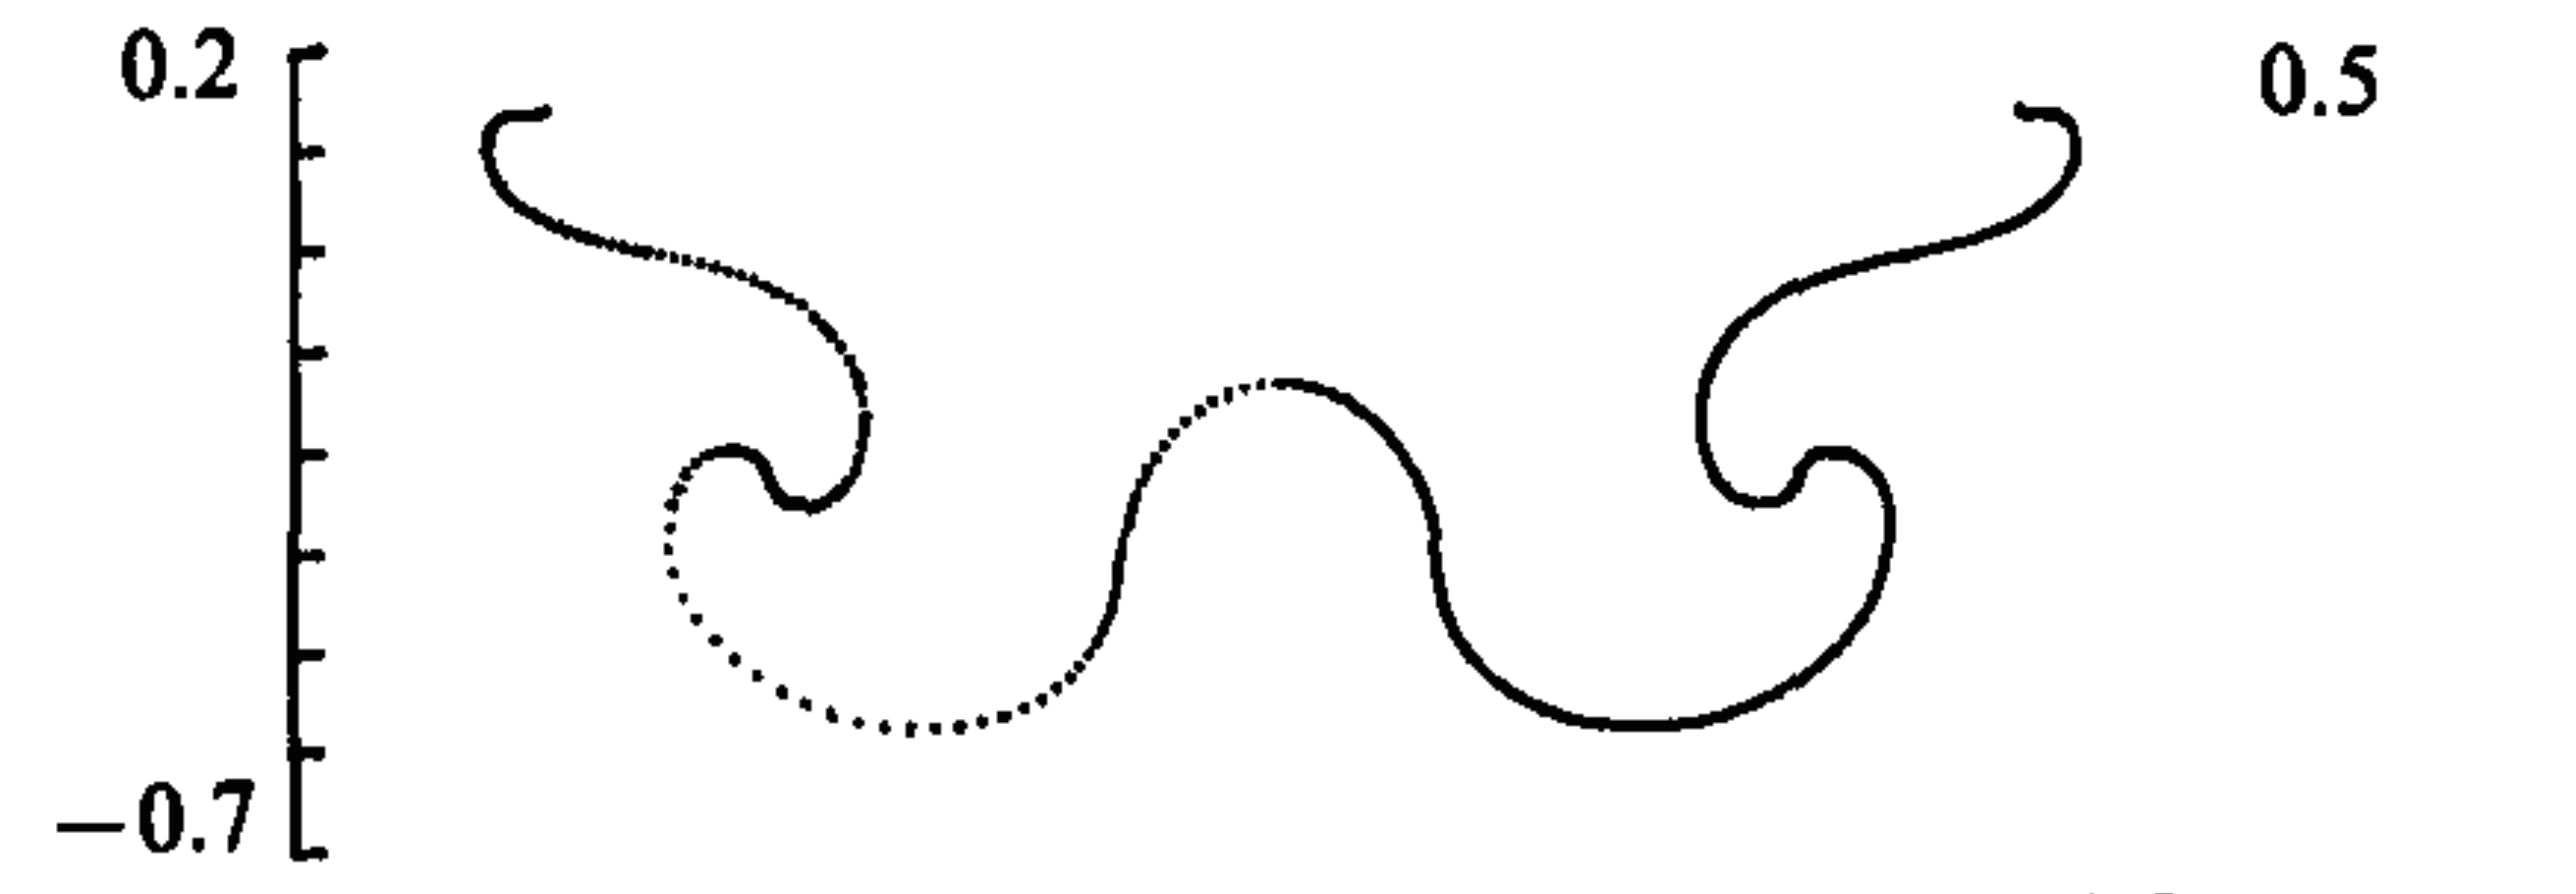
\includegraphics[width=2in,height=1.in]{fuse3.png}}

	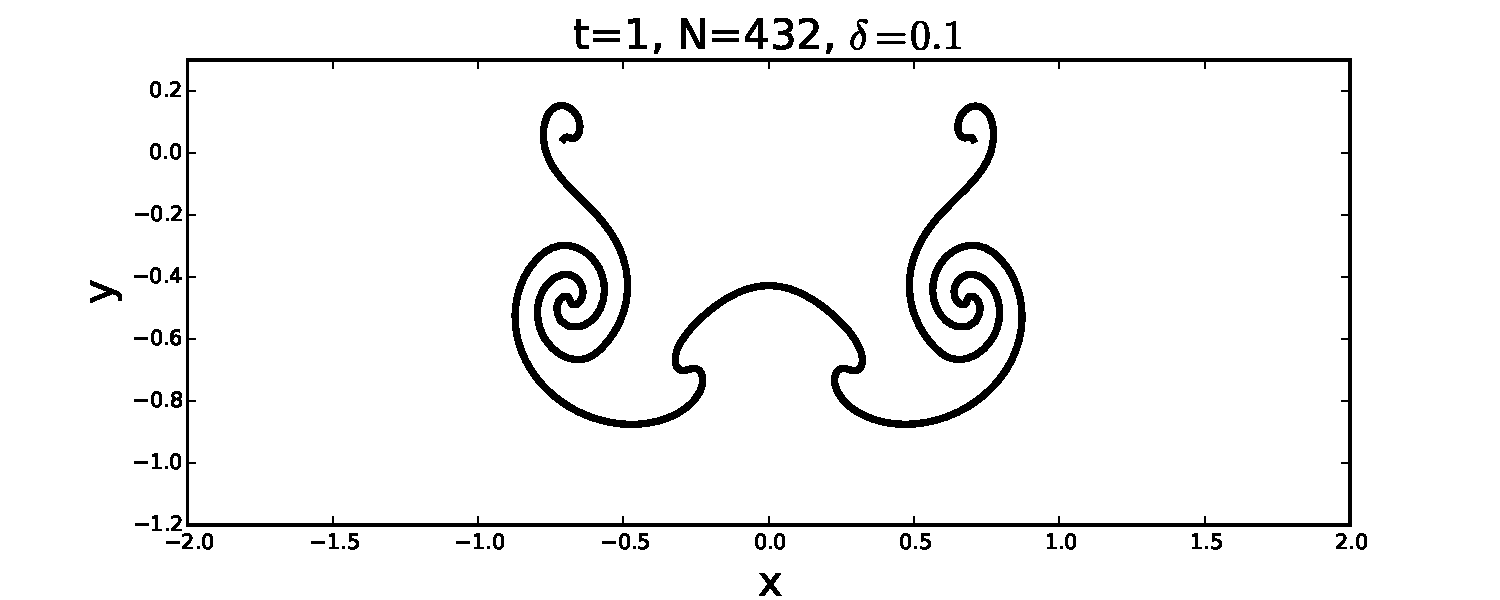
\includegraphics[width=3in,height=1.33in]{FU4.pdf}\raisebox{0.15\height}{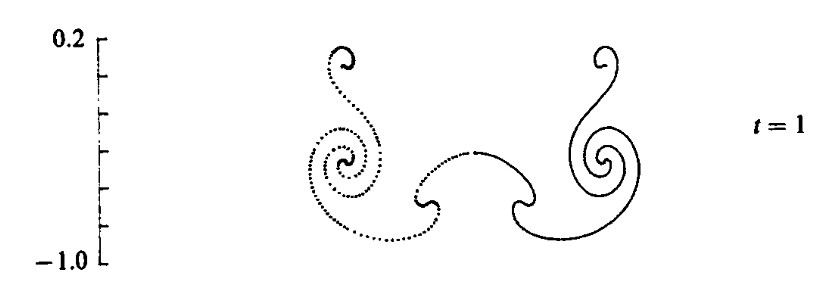
\includegraphics[width=2in,height=1.in]{fuse4.png}}

	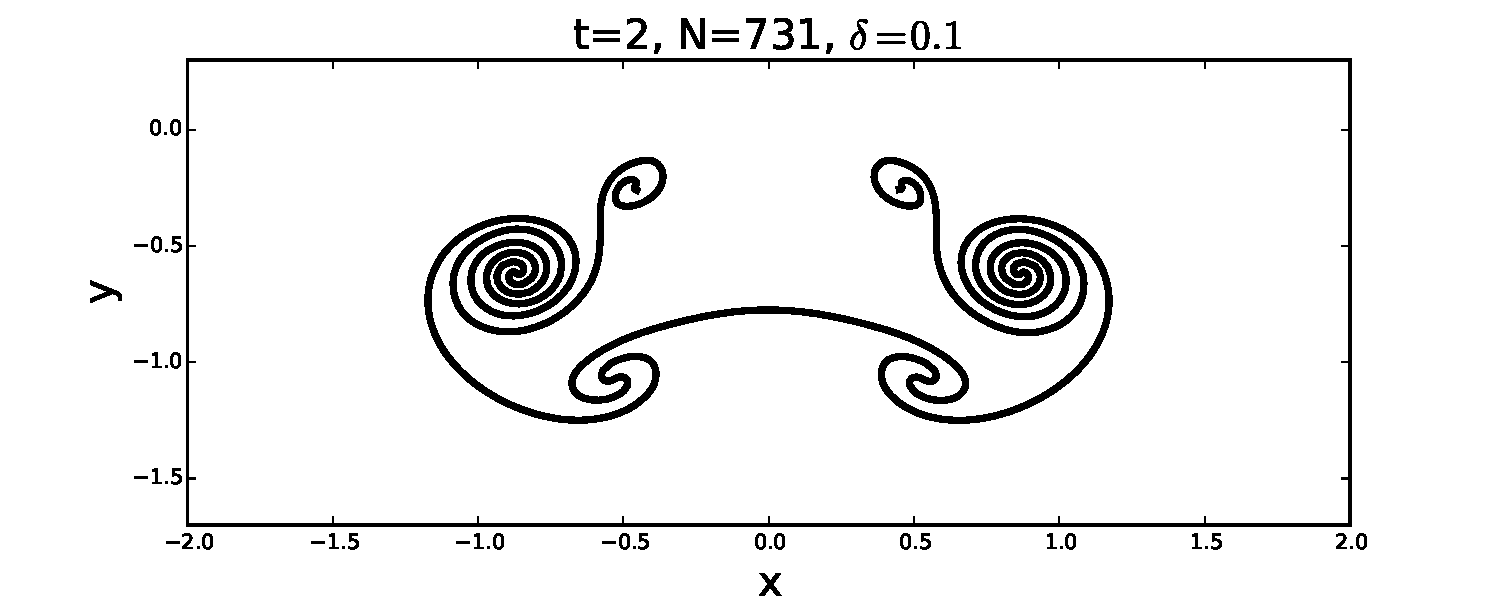
\includegraphics[width=3in,height=1.33in]{FU5.pdf}\raisebox{0.15\height}{\includegraphics[width=2in,height=1.in]{fuse5.png}}
		\includegraphics[width=3in,height=1.33in]{FU6.pdf}\raisebox{0.15\height}{\includegraphics[width=2in,height=1.in]{fuse6.png}}
			\includegraphics[width=3in,height=1.33in]{FU7.pdf}\raisebox{0.15\height}{\includegraphics[width=2in,height=1.in]{fuse7.png}}
\end{center}
\caption{Roll-up in the simulated fuselage flap, with $N=200$, $\delta=0.1$ and $\Delta t=0.02$}
\end{figure}
\clearpage
\section{References}
$[1]$ R. Krasny, Desingularization of Periodic Vortex Sheet Roll-up, Journal of Computational Physics 65, 292-313 (1986)\\ 
$[2]$ R. Krasny, Computation of vortex sheet roll-up in the Trefftz plane, J. Fluid Mechanics, vol. 184, pp. 123-155  (1987)  
\end{document}


